%% ICT Express research paper -- Draft v5 (11 Nov 2026): revised after internal re-review of draft v4
%% Class and options from the official ICT Express sample manuscript
%% ("ICT Express Submission Template_191231.zip", linked from the journal's Guide for Authors).
\documentclass[final,3p,times,twocolumn]{elsarticle}

\usepackage{graphicx, amsmath, amssymb, algorithm, algpseudocode}
\usepackage{booktabs}
\usepackage[utf8]{inputenc}
\usepackage[english]{babel}
\usepackage{tikz}
\usetikzlibrary{positioning,arrows.meta,fit,calc,shapes.multipart}
\usepackage[hyphens]{url}
\usepackage{hyperref}
\hypersetup{colorlinks=true, linkcolor=black, citecolor=black, filecolor=black, urlcolor=blue}
\usepackage{caption}
\captionsetup{justification=raggedright, singlelinecheck=false, font=small}
\captionsetup[table]{labelformat=simple, labelsep=newline}
\captionsetup[figure]{labelformat=simple, labelsep=period}
\usepackage{microtype}
\usepackage{array}
\newcolumntype{L}[1]{>{\raggedright\arraybackslash\hspace{0pt}}p{#1}}
\setlength{\textfloatsep}{8pt plus 2pt minus 2pt}
\setlength{\floatsep}{6pt plus 2pt minus 2pt}
\setlength{\dbltextfloatsep}{8pt plus 2pt minus 2pt}
\newtheorem{claim}{Claim}
\newcommand{\Sa}{S1a}\newcommand{\Sb}{S1b}
% auto-generated by paper_numbers_v5.py (v4 macros + v5 additions) — do not edit by hand
% names may contain digits, so they are stored via \csname and used as \Nm{Name}
\providecommand{\Nm}[1]{\ifcsname N#1\endcsname\csname N#1\endcsname\else\textbf{??#1}\fi}
\expandafter\def\csname NGasStwoMin\endcsname{49,675}
\expandafter\def\csname NGasStwoMax\endcsname{49,687}
\expandafter\def\csname NGasSthreeMin\endcsname{49,703}
\expandafter\def\csname NGasSthreeMax\endcsname{49,709}
\expandafter\def\csname NGasEventStwoMin\endcsname{28,996}
\expandafter\def\csname NGasEventStwoMax\endcsname{29,008}
\expandafter\def\csname NBytesEventStwo\endcsname{164}
\expandafter\def\csname NGasEventSthreeMin\endcsname{29,002}
\expandafter\def\csname NGasEventSthreeMax\endcsname{29,008}
\expandafter\def\csname NBytesEventSthree\endcsname{164}
\expandafter\def\csname NGasSoneaK10\endcsname{446,326}
\expandafter\def\csname NBytesSoneaK10\endcsname{1,320}
\expandafter\def\csname NGasSonebK10\endcsname{250,743}
\expandafter\def\csname NBytesSonebK10\endcsname{740}
\expandafter\def\csname NGasStwoK10\endcsname{49,687}
\expandafter\def\csname NBytesStwoK10\endcsname{100}
\expandafter\def\csname NGasSthreeK10\endcsname{49,709}
\expandafter\def\csname NBytesSthreeK10\endcsname{100}
\expandafter\def\csname NGasSoneaK50\endcsname{2,231,654}
\expandafter\def\csname NBytesSoneaK50\endcsname{6,600}
\expandafter\def\csname NGasSonebK50\endcsname{1,165,471}
\expandafter\def\csname NBytesSonebK50\endcsname{3,300}
\expandafter\def\csname NGasStwoK50\endcsname{49,687}
\expandafter\def\csname NBytesStwoK50\endcsname{100}
\expandafter\def\csname NGasSthreeK50\endcsname{49,709}
\expandafter\def\csname NBytesSthreeK50\endcsname{100}
\expandafter\def\csname NGasSoneaK100\endcsname{4,463,344}
\expandafter\def\csname NBytesSoneaK100\endcsname{13,200}
\expandafter\def\csname NGasSonebK100\endcsname{2,308,911}
\expandafter\def\csname NBytesSonebK100\endcsname{6,500}
\expandafter\def\csname NGasStwoK100\endcsname{49,687}
\expandafter\def\csname NBytesStwoK100\endcsname{100}
\expandafter\def\csname NGasSthreeK100\endcsname{49,709}
\expandafter\def\csname NBytesSthreeK100\endcsname{100}
\expandafter\def\csname NGasSoneaK500\endcsname{22,319,606}
\expandafter\def\csname NBytesSoneaK500\endcsname{66,000}
\expandafter\def\csname NGasSonebK500\endcsname{11,456,269}
\expandafter\def\csname NBytesSonebK500\endcsname{32,100}
\expandafter\def\csname NGasStwoK500\endcsname{49,687}
\expandafter\def\csname NBytesStwoK500\endcsname{100}
\expandafter\def\csname NGasSthreeK500\endcsname{49,703}
\expandafter\def\csname NBytesSthreeK500\endcsname{100}
\expandafter\def\csname NGasSoneaK1000\endcsname{44,642,440}
\expandafter\def\csname NBytesSoneaK1000\endcsname{132,000}
\expandafter\def\csname NGasSonebK1000\endcsname{22,890,627}
\expandafter\def\csname NBytesSonebK1000\endcsname{64,100}
\expandafter\def\csname NGasStwoK1000\endcsname{49,675}
\expandafter\def\csname NBytesStwoK1000\endcsname{100}
\expandafter\def\csname NGasSthreeK1000\endcsname{49,709}
\expandafter\def\csname NBytesSthreeK1000\endcsname{100}
\expandafter\def\csname NFitSoneaSlope\endcsname{44,643}
\expandafter\def\csname NFitSoneaIntercept\endcsname{-663.4}
\expandafter\def\csname NFitSoneaEventSlope\endcsname{24,190}
\expandafter\def\csname NFitSoneaEventIntercept\endcsname{-663.4}
\expandafter\def\csname NFitSonebSlope\endcsname{22,869}
\expandafter\def\csname NFitSonebIntercept\endcsname{22,042.5}
\expandafter\def\csname NFitSonebEventSlope\endcsname{1,276}
\expandafter\def\csname NFitSonebEventIntercept\endcsname{22,178.7}
\expandafter\def\csname NGasStwoRoundOne\endcsname{66,787}
\expandafter\def\csname NGasSthreeRoundOne\endcsname{66,809}
\expandafter\def\csname NEipSonebKcap\endcsname{733}
\expandafter\def\csname NTchainStwoSthreeMin\endcsname{9.6}
\expandafter\def\csname NTchainStwoSthreeMax\endcsname{11.8}
\expandafter\def\csname NTchainSoneaK10\endcsname{101.2}
\expandafter\def\csname NTtotalSoneaK10\endcsname{101.2}
\expandafter\def\csname NTchainSonebK10\endcsname{10.0}
\expandafter\def\csname NTtotalSonebK10\endcsname{10.0}
\expandafter\def\csname NTchainStwoK10\endcsname{10.3}
\expandafter\def\csname NTtotalStwoK10\endcsname{10.3}
\expandafter\def\csname NTchainSthreeK10\endcsname{9.6}
\expandafter\def\csname NTtotalSthreeK10\endcsname{26.8}
\expandafter\def\csname NTchainSthreeFourK10\endcsname{10.3}
\expandafter\def\csname NTtotalSthreeFourK10\endcsname{32.3}
\expandafter\def\csname NTchainSthreeFlatK10\endcsname{10.4}
\expandafter\def\csname NTtotalSthreeFlatK10\endcsname{32.4}
\expandafter\def\csname NTblobK10\endcsname{60.1}
\expandafter\def\csname NTverSoneK10\endcsname{8.8}
\expandafter\def\csname NTverSoneK10Qone\endcsname{8.4}
\expandafter\def\csname NTverSoneK10Qthree\endcsname{9.5}
\expandafter\def\csname NProofSoneK10\endcsname{32}
\expandafter\def\csname NNverSoneK10\endcsname{100}
\expandafter\def\csname NTidxSoneK10\endcsname{0.4}
\expandafter\def\csname NNfetchSoneK10\endcsname{0}
\expandafter\def\csname NTverStwoK10\endcsname{8.9}
\expandafter\def\csname NTverStwoK10Qone\endcsname{8.6}
\expandafter\def\csname NTverStwoK10Qthree\endcsname{9.7}
\expandafter\def\csname NProofStwoK10\endcsname{119}
\expandafter\def\csname NNverStwoK10\endcsname{100}
\expandafter\def\csname NTidxStwoK10\endcsname{0.5}
\expandafter\def\csname NNfetchStwoK10\endcsname{0}
\expandafter\def\csname NTverStwosigK10\endcsname{14.1}
\expandafter\def\csname NTverStwosigK10Qone\endcsname{13.7}
\expandafter\def\csname NTverStwosigK10Qthree\endcsname{15.4}
\expandafter\def\csname NProofStwosigK10\endcsname{224}
\expandafter\def\csname NNverStwosigK10\endcsname{100}
\expandafter\def\csname NTidxStwosigK10\endcsname{0.4}
\expandafter\def\csname NNfetchStwosigK10\endcsname{0}
\expandafter\def\csname NTverSthreeK10\endcsname{18.4}
\expandafter\def\csname NTverSthreeK10Qone\endcsname{17.8}
\expandafter\def\csname NTverSthreeK10Qthree\endcsname{20.3}
\expandafter\def\csname NProofSthreeK10\endcsname{894}
\expandafter\def\csname NNverSthreeK10\endcsname{100}
\expandafter\def\csname NTidxSthreeK10\endcsname{0.0}
\expandafter\def\csname NNfetchSthreeK10\endcsname{2}
\expandafter\def\csname NTverSthreeFourK10\endcsname{18.9}
\expandafter\def\csname NTverSthreeFourK10Qone\endcsname{18.5}
\expandafter\def\csname NTverSthreeFourK10Qthree\endcsname{20.6}
\expandafter\def\csname NProofSthreeFourK10\endcsname{779}
\expandafter\def\csname NNverSthreeFourK10\endcsname{100}
\expandafter\def\csname NTidxSthreeFourK10\endcsname{0.0}
\expandafter\def\csname NNfetchSthreeFourK10\endcsname{3}
\expandafter\def\csname NTverSthreeFlatK10\endcsname{18.6}
\expandafter\def\csname NTverSthreeFlatK10Qone\endcsname{17.8}
\expandafter\def\csname NTverSthreeFlatK10Qthree\endcsname{19.9}
\expandafter\def\csname NProofSthreeFlatK10\endcsname{894}
\expandafter\def\csname NNverSthreeFlatK10\endcsname{100}
\expandafter\def\csname NTidxSthreeFlatK10\endcsname{0.0}
\expandafter\def\csname NNfetchSthreeFlatK10\endcsname{2}
\expandafter\def\csname NTchainSoneaK50\endcsname{562.7}
\expandafter\def\csname NTtotalSoneaK50\endcsname{562.7}
\expandafter\def\csname NTchainSonebK50\endcsname{13.4}
\expandafter\def\csname NTtotalSonebK50\endcsname{13.4}
\expandafter\def\csname NTchainStwoK50\endcsname{11.8}
\expandafter\def\csname NTtotalStwoK50\endcsname{12.1}
\expandafter\def\csname NTchainSthreeK50\endcsname{10.7}
\expandafter\def\csname NTtotalSthreeK50\endcsname{95.7}
\expandafter\def\csname NTchainSthreeFourK50\endcsname{10.5}
\expandafter\def\csname NTtotalSthreeFourK50\endcsname{118.8}
\expandafter\def\csname NTchainSthreeFlatK50\endcsname{11.0}
\expandafter\def\csname NTtotalSthreeFlatK50\endcsname{104.9}
\expandafter\def\csname NTblobK50\endcsname{274.5}
\expandafter\def\csname NTverSoneK50\endcsname{9.0}
\expandafter\def\csname NTverSoneK50Qone\endcsname{8.5}
\expandafter\def\csname NTverSoneK50Qthree\endcsname{9.7}
\expandafter\def\csname NProofSoneK50\endcsname{32}
\expandafter\def\csname NNverSoneK50\endcsname{500}
\expandafter\def\csname NTidxSoneK50\endcsname{0.4}
\expandafter\def\csname NNfetchSoneK50\endcsname{0}
\expandafter\def\csname NTverStwoK50\endcsname{8.9}
\expandafter\def\csname NTverStwoK50Qone\endcsname{8.4}
\expandafter\def\csname NTverStwoK50Qthree\endcsname{9.6}
\expandafter\def\csname NProofStwoK50\endcsname{192}
\expandafter\def\csname NNverStwoK50\endcsname{500}
\expandafter\def\csname NTidxStwoK50\endcsname{0.4}
\expandafter\def\csname NNfetchStwoK50\endcsname{0}
\expandafter\def\csname NTverStwosigK50\endcsname{14.5}
\expandafter\def\csname NTverStwosigK50Qone\endcsname{13.8}
\expandafter\def\csname NTverStwosigK50Qthree\endcsname{15.9}
\expandafter\def\csname NProofStwosigK50\endcsname{297}
\expandafter\def\csname NNverStwosigK50\endcsname{500}
\expandafter\def\csname NTidxStwosigK50\endcsname{0.4}
\expandafter\def\csname NNfetchStwosigK50\endcsname{0}
\expandafter\def\csname NTverSthreeK50\endcsname{21.2}
\expandafter\def\csname NTverSthreeK50Qone\endcsname{20.2}
\expandafter\def\csname NTverSthreeK50Qthree\endcsname{23.2}
\expandafter\def\csname NProofSthreeK50\endcsname{1,307}
\expandafter\def\csname NNverSthreeK50\endcsname{500}
\expandafter\def\csname NTidxSthreeK50\endcsname{0.0}
\expandafter\def\csname NNfetchSthreeK50\endcsname{3}
\expandafter\def\csname NTverSthreeFourK50\endcsname{21.5}
\expandafter\def\csname NTverSthreeFourK50Qone\endcsname{20.5}
\expandafter\def\csname NTverSthreeFourK50Qthree\endcsname{23.4}
\expandafter\def\csname NProofSthreeFourK50\endcsname{1,019}
\expandafter\def\csname NNverSthreeFourK50\endcsname{500}
\expandafter\def\csname NTidxSthreeFourK50\endcsname{0.0}
\expandafter\def\csname NNfetchSthreeFourK50\endcsname{4}
\expandafter\def\csname NTverSthreeFlatK50\endcsname{23.8}
\expandafter\def\csname NTverSthreeFlatK50Qone\endcsname{22.9}
\expandafter\def\csname NTverSthreeFlatK50Qthree\endcsname{26.3}
\expandafter\def\csname NProofSthreeFlatK50\endcsname{2,537}
\expandafter\def\csname NNverSthreeFlatK50\endcsname{500}
\expandafter\def\csname NTidxSthreeFlatK50\endcsname{0.0}
\expandafter\def\csname NNfetchSthreeFlatK50\endcsname{2}
\expandafter\def\csname NTchainSoneaK100\endcsname{1,007.5}
\expandafter\def\csname NTtotalSoneaK100\endcsname{1,007.6}
\expandafter\def\csname NTchainSonebK100\endcsname{19.7}
\expandafter\def\csname NTtotalSonebK100\endcsname{19.8}
\expandafter\def\csname NTchainStwoK100\endcsname{10.1}
\expandafter\def\csname NTtotalStwoK100\endcsname{10.5}
\expandafter\def\csname NTchainSthreeK100\endcsname{11.1}
\expandafter\def\csname NTtotalSthreeK100\endcsname{168.5}
\expandafter\def\csname NTchainSthreeFourK100\endcsname{10.2}
\expandafter\def\csname NTtotalSthreeFourK100\endcsname{204.6}
\expandafter\def\csname NTchainSthreeFlatK100\endcsname{10.1}
\expandafter\def\csname NTtotalSthreeFlatK100\endcsname{187.3}
\expandafter\def\csname NTblobK100\endcsname{526.8}
\expandafter\def\csname NTverSoneK100\endcsname{9.3}
\expandafter\def\csname NTverSoneK100Qone\endcsname{8.7}
\expandafter\def\csname NTverSoneK100Qthree\endcsname{10.1}
\expandafter\def\csname NProofSoneK100\endcsname{32}
\expandafter\def\csname NNverSoneK100\endcsname{1,000}
\expandafter\def\csname NTidxSoneK100\endcsname{0.4}
\expandafter\def\csname NNfetchSoneK100\endcsname{0}
\expandafter\def\csname NTverStwoK100\endcsname{8.8}
\expandafter\def\csname NTverStwoK100Qone\endcsname{8.3}
\expandafter\def\csname NTverStwoK100Qthree\endcsname{9.5}
\expandafter\def\csname NProofStwoK100\endcsname{224}
\expandafter\def\csname NNverStwoK100\endcsname{1,000}
\expandafter\def\csname NTidxStwoK100\endcsname{0.4}
\expandafter\def\csname NNfetchStwoK100\endcsname{0}
\expandafter\def\csname NTverStwosigK100\endcsname{14.1}
\expandafter\def\csname NTverStwosigK100Qone\endcsname{13.4}
\expandafter\def\csname NTverStwosigK100Qthree\endcsname{15.7}
\expandafter\def\csname NProofStwosigK100\endcsname{329}
\expandafter\def\csname NNverStwosigK100\endcsname{1,000}
\expandafter\def\csname NTidxStwosigK100\endcsname{0.4}
\expandafter\def\csname NNfetchStwosigK100\endcsname{0}
\expandafter\def\csname NTverSthreeK100\endcsname{21.9}
\expandafter\def\csname NTverSthreeK100Qone\endcsname{20.7}
\expandafter\def\csname NTverSthreeK100Qthree\endcsname{24.2}
\expandafter\def\csname NProofSthreeK100\endcsname{1,434}
\expandafter\def\csname NNverSthreeK100\endcsname{1,000}
\expandafter\def\csname NTidxSthreeK100\endcsname{0.0}
\expandafter\def\csname NNfetchSthreeK100\endcsname{3}
\expandafter\def\csname NTverSthreeFourK100\endcsname{23.2}
\expandafter\def\csname NTverSthreeFourK100Qone\endcsname{22.0}
\expandafter\def\csname NTverSthreeFourK100Qthree\endcsname{25.3}
\expandafter\def\csname NProofSthreeFourK100\endcsname{1,115}
\expandafter\def\csname NNverSthreeFourK100\endcsname{1,000}
\expandafter\def\csname NTidxSthreeFourK100\endcsname{0.0}
\expandafter\def\csname NNfetchSthreeFourK100\endcsname{5}
\expandafter\def\csname NTverSthreeFlatK100\endcsname{30.2}
\expandafter\def\csname NTverSthreeFlatK100Qone\endcsname{28.5}
\expandafter\def\csname NTverSthreeFlatK100Qthree\endcsname{33.2}
\expandafter\def\csname NProofSthreeFlatK100\endcsname{4,587}
\expandafter\def\csname NNverSthreeFlatK100\endcsname{1,000}
\expandafter\def\csname NTidxSthreeFlatK100\endcsname{0.0}
\expandafter\def\csname NNfetchSthreeFlatK100\endcsname{2}
\expandafter\def\csname NTchainSoneaK500\endcsname{5,323.4}
\expandafter\def\csname NTtotalSoneaK500\endcsname{5,323.5}
\expandafter\def\csname NTchainSonebK500\endcsname{141.7}
\expandafter\def\csname NTtotalSonebK500\endcsname{141.9}
\expandafter\def\csname NTchainStwoK500\endcsname{10.4}
\expandafter\def\csname NTtotalStwoK500\endcsname{13.0}
\expandafter\def\csname NTchainSthreeK500\endcsname{10.4}
\expandafter\def\csname NTtotalSthreeK500\endcsname{782.2}
\expandafter\def\csname NTchainSthreeFourK500\endcsname{11.7}
\expandafter\def\csname NTtotalSthreeFourK500\endcsname{1,030.6}
\expandafter\def\csname NTchainSthreeFlatK500\endcsname{10.3}
\expandafter\def\csname NTtotalSthreeFlatK500\endcsname{856.0}
\expandafter\def\csname NTblobK500\endcsname{2,694.1}
\expandafter\def\csname NTverSoneK500\endcsname{9.3}
\expandafter\def\csname NTverSoneK500Qone\endcsname{8.8}
\expandafter\def\csname NTverSoneK500Qthree\endcsname{10.1}
\expandafter\def\csname NProofSoneK500\endcsname{32}
\expandafter\def\csname NNverSoneK500\endcsname{2,000}
\expandafter\def\csname NTidxSoneK500\endcsname{0.4}
\expandafter\def\csname NNfetchSoneK500\endcsname{0}
\expandafter\def\csname NTverStwoK500\endcsname{8.8}
\expandafter\def\csname NTverStwoK500Qone\endcsname{8.3}
\expandafter\def\csname NTverStwoK500Qthree\endcsname{9.6}
\expandafter\def\csname NProofStwoK500\endcsname{291}
\expandafter\def\csname NNverStwoK500\endcsname{2,000}
\expandafter\def\csname NTidxStwoK500\endcsname{0.4}
\expandafter\def\csname NNfetchStwoK500\endcsname{0}
\expandafter\def\csname NTverStwosigK500\endcsname{14.1}
\expandafter\def\csname NTverStwosigK500Qone\endcsname{13.4}
\expandafter\def\csname NTverStwosigK500Qthree\endcsname{15.3}
\expandafter\def\csname NProofStwosigK500\endcsname{396}
\expandafter\def\csname NNverStwosigK500\endcsname{2,000}
\expandafter\def\csname NTidxStwosigK500\endcsname{0.4}
\expandafter\def\csname NNfetchStwosigK500\endcsname{0}
\expandafter\def\csname NTverSthreeK500\endcsname{25.1}
\expandafter\def\csname NTverSthreeK500Qone\endcsname{24.0}
\expandafter\def\csname NTverSthreeK500Qthree\endcsname{27.4}
\expandafter\def\csname NProofSthreeK500\endcsname{1,927}
\expandafter\def\csname NNverSthreeK500\endcsname{2,000}
\expandafter\def\csname NTidxSthreeK500\endcsname{0.0}
\expandafter\def\csname NNfetchSthreeK500\endcsname{4}
\expandafter\def\csname NTverSthreeFourK500\endcsname{24.9}
\expandafter\def\csname NTverSthreeFourK500Qone\endcsname{23.8}
\expandafter\def\csname NTverSthreeFourK500Qthree\endcsname{26.9}
\expandafter\def\csname NProofSthreeFourK500\endcsname{1,324}
\expandafter\def\csname NNverSthreeFourK500\endcsname{2,000}
\expandafter\def\csname NTidxSthreeFourK500\endcsname{0.0}
\expandafter\def\csname NNfetchSthreeFourK500\endcsname{6}
\expandafter\def\csname NTverSthreeFlatK500\endcsname{80.8}
\expandafter\def\csname NTverSthreeFlatK500Qone\endcsname{77.5}
\expandafter\def\csname NTverSthreeFlatK500Qthree\endcsname{88.7}
\expandafter\def\csname NProofSthreeFlatK500\endcsname{20,991}
\expandafter\def\csname NNverSthreeFlatK500\endcsname{2,000}
\expandafter\def\csname NTidxSthreeFlatK500\endcsname{0.0}
\expandafter\def\csname NNfetchSthreeFlatK500\endcsname{2}
\expandafter\def\csname NTchainSoneaK1000\endcsname{10,435.8}
\expandafter\def\csname NTtotalSoneaK1000\endcsname{10,436.0}
\expandafter\def\csname NTchainSonebK1000\endcsname{166.2}
\expandafter\def\csname NTtotalSonebK1000\endcsname{166.5}
\expandafter\def\csname NTchainStwoK1000\endcsname{10.2}
\expandafter\def\csname NTtotalStwoK1000\endcsname{16.9}
\expandafter\def\csname NTchainSthreeK1000\endcsname{10.7}
\expandafter\def\csname NTtotalSthreeK1000\endcsname{1,602.3}
\expandafter\def\csname NTchainSthreeFourK1000\endcsname{11.1}
\expandafter\def\csname NTtotalSthreeFourK1000\endcsname{2,075.5}
\expandafter\def\csname NTchainSthreeFlatK1000\endcsname{11.2}
\expandafter\def\csname NTtotalSthreeFlatK1000\endcsname{1,758.0}
\expandafter\def\csname NTblobK1000\endcsname{5,534.7}
\expandafter\def\csname NTverSoneK1000\endcsname{9.4}
\expandafter\def\csname NTverSoneK1000Qone\endcsname{8.8}
\expandafter\def\csname NTverSoneK1000Qthree\endcsname{10.3}
\expandafter\def\csname NProofSoneK1000\endcsname{32}
\expandafter\def\csname NNverSoneK1000\endcsname{2,000}
\expandafter\def\csname NTidxSoneK1000\endcsname{0.4}
\expandafter\def\csname NNfetchSoneK1000\endcsname{0}
\expandafter\def\csname NTverStwoK1000\endcsname{8.8}
\expandafter\def\csname NTverStwoK1000Qone\endcsname{8.3}
\expandafter\def\csname NTverStwoK1000Qthree\endcsname{9.7}
\expandafter\def\csname NProofStwoK1000\endcsname{323}
\expandafter\def\csname NNverStwoK1000\endcsname{2,000}
\expandafter\def\csname NTidxStwoK1000\endcsname{0.4}
\expandafter\def\csname NNfetchStwoK1000\endcsname{0}
\expandafter\def\csname NTverStwosigK1000\endcsname{14.2}
\expandafter\def\csname NTverStwosigK1000Qone\endcsname{13.5}
\expandafter\def\csname NTverStwosigK1000Qthree\endcsname{15.8}
\expandafter\def\csname NProofStwosigK1000\endcsname{428}
\expandafter\def\csname NNverStwosigK1000\endcsname{2,000}
\expandafter\def\csname NTidxStwosigK1000\endcsname{0.4}
\expandafter\def\csname NNfetchStwosigK1000\endcsname{0}
\expandafter\def\csname NTverSthreeK1000\endcsname{25.6}
\expandafter\def\csname NTverSthreeK1000Qone\endcsname{24.5}
\expandafter\def\csname NTverSthreeK1000Qthree\endcsname{28.1}
\expandafter\def\csname NProofSthreeK1000\endcsname{2,001}
\expandafter\def\csname NNverSthreeK1000\endcsname{2,000}
\expandafter\def\csname NTidxSthreeK1000\endcsname{0.0}
\expandafter\def\csname NNfetchSthreeK1000\endcsname{4}
\expandafter\def\csname NTverSthreeFourK1000\endcsname{25.3}
\expandafter\def\csname NTverSthreeFourK1000Qone\endcsname{24.3}
\expandafter\def\csname NTverSthreeFourK1000Qthree\endcsname{27.9}
\expandafter\def\csname NProofSthreeFourK1000\endcsname{1,405}
\expandafter\def\csname NNverSthreeFourK1000\endcsname{2,000}
\expandafter\def\csname NTidxSthreeFourK1000\endcsname{0.0}
\expandafter\def\csname NNfetchSthreeFourK1000\endcsname{6}
\expandafter\def\csname NTverSthreeFlatK1000\endcsname{145.4}
\expandafter\def\csname NTverSthreeFlatK1000Qone\endcsname{139.0}
\expandafter\def\csname NTverSthreeFlatK1000Qthree\endcsname{158.6}
\expandafter\def\csname NProofSthreeFlatK1000\endcsname{41,491}
\expandafter\def\csname NNverSthreeFlatK1000\endcsname{2,000}
\expandafter\def\csname NTidxSthreeFlatK1000\endcsname{0.0}
\expandafter\def\csname NNfetchSthreeFlatK1000\endcsname{2}
\expandafter\def\csname NPszStwoK100\endcsname{224}
\expandafter\def\csname NPszStwosigK100\endcsname{329}
\expandafter\def\csname NPszSthreeK100\endcsname{1,355}
\expandafter\def\csname NPszSthreeFourK100\endcsname{1,036}
\expandafter\def\csname NPszSthreeFlatK100\endcsname{4,508}
\expandafter\def\csname NPszStwoK500\endcsname{291}
\expandafter\def\csname NPszStwosigK500\endcsname{396}
\expandafter\def\csname NPszSthreeK500\endcsname{1,847}
\expandafter\def\csname NPszSthreeFourK500\endcsname{1,245}
\expandafter\def\csname NPszSthreeFlatK500\endcsname{20,912}
\expandafter\def\csname NPszStwoK1000\endcsname{323}
\expandafter\def\csname NPszStwosigK1000\endcsname{428}
\expandafter\def\csname NPszSthreeK1000\endcsname{1,921}
\expandafter\def\csname NPszSthreeFourK1000\endcsname{1,325}
\expandafter\def\csname NPszSthreeFlatK1000\endcsname{41,412}
\expandafter\def\csname NTamperRuns\endcsname{53}
\expandafter\def\csname NTamperT1S1\endcsname{53/53}
\expandafter\def\csname NTamperT1S2\endcsname{53/53}
\expandafter\def\csname NTamperT1S2sig\endcsname{53/53}
\expandafter\def\csname NTamperT1S3\endcsname{53/53}
\expandafter\def\csname NTamperT2S1\endcsname{53/53}
\expandafter\def\csname NTamperT2S2\endcsname{53/53}
\expandafter\def\csname NTamperT2S2sig\endcsname{53/53}
\expandafter\def\csname NTamperT2S3\endcsname{53/53}
\expandafter\def\csname NTamperT3aS1\endcsname{53/53}
\expandafter\def\csname NTamperT3aS2\endcsname{53/53}
\expandafter\def\csname NTamperT3aS2sig\endcsname{53/53}
\expandafter\def\csname NTamperT3aS3\endcsname{53/53}
\expandafter\def\csname NTamperT3bS1\endcsname{0/53}
\expandafter\def\csname NTamperT3bS2\endcsname{0/53}
\expandafter\def\csname NTamperT3bS2sig\endcsname{53/53}
\expandafter\def\csname NTamperT3bS3\endcsname{53/53}
\expandafter\def\csname NTamperT4S1guard\endcsname{53/53}
\expandafter\def\csname NTamperT4S2\endcsname{53/53}
\expandafter\def\csname NTamperT4S2sig\endcsname{53/53}
\expandafter\def\csname NTamperT4S3\endcsname{53/53}
\expandafter\def\csname NTamperT5S1\endcsname{53/53}
\expandafter\def\csname NTamperT5S2\endcsname{53/53}
\expandafter\def\csname NTamperT5S2sig\endcsname{53/53}
\expandafter\def\csname NTamperT5S3\endcsname{53/53}
\expandafter\def\csname NTamperT6S1\endcsname{0/53}
\expandafter\def\csname NTamperT6S2\endcsname{0/53}
\expandafter\def\csname NTamperT6S2sig\endcsname{53/53}
\expandafter\def\csname NTamperT6S3\endcsname{53/53}
\expandafter\def\csname NGasGapK10\endcsname{22}
\expandafter\def\csname NGasEventStwoK10\endcsname{29,008}
\expandafter\def\csname NGasEventSthreeK10\endcsname{29,008}
\expandafter\def\csname NGasGapK50\endcsname{22}
\expandafter\def\csname NGasEventStwoK50\endcsname{29,008}
\expandafter\def\csname NGasEventSthreeK50\endcsname{29,008}
\expandafter\def\csname NGasGapK100\endcsname{22}
\expandafter\def\csname NGasEventStwoK100\endcsname{29,008}
\expandafter\def\csname NGasEventSthreeK100\endcsname{29,008}
\expandafter\def\csname NGasGapK500\endcsname{16}
\expandafter\def\csname NGasEventStwoK500\endcsname{29,008}
\expandafter\def\csname NGasEventSthreeK500\endcsname{29,002}
\expandafter\def\csname NGasGapK1000\endcsname{34}
\expandafter\def\csname NGasEventStwoK1000\endcsname{28,996}
\expandafter\def\csname NGasEventSthreeK1000\endcsname{29,008}
\expandafter\def\csname NGasGapMedMin\endcsname{16}
\expandafter\def\csname NGasGapMedMax\endcsname{34}
\expandafter\def\csname NGasGapPairs\endcsname{922}
\expandafter\def\csname NGasGapRoundMin\endcsname{$-$2}
\expandafter\def\csname NGasGapRoundMax\endcsname{46}
\expandafter\def\csname NDagSizeB\endcsname{424,356}
\expandafter\def\csname NDagTimeout\endcsname{5}
\expandafter\def\csname NDagWallMin\endcsname{5.8}
\expandafter\def\csname NDagOkAll\endcsname{800/800}
\expandafter\def\csname NDagNaudKonehundred\endcsname{100}
\expandafter\def\csname NDagMetaMedKonehundredBsixteen\endcsname{60.3}
\expandafter\def\csname NDagMetaQoneKonehundredBsixteen\endcsname{59.1}
\expandafter\def\csname NDagMetaQthreeKonehundredBsixteen\endcsname{60.9}
\expandafter\def\csname NDagFullMedKonehundredBsixteen\endcsname{136.0}
\expandafter\def\csname NDagFullQoneKonehundredBsixteen\endcsname{134.9}
\expandafter\def\csname NDagFullQthreeKonehundredBsixteen\endcsname{137.1}
\expandafter\def\csname NDagOkKonehundredBsixteen\endcsname{200/200}
\expandafter\def\csname NDagBlocksKonehundredBsixteen\endcsname{3}
\expandafter\def\csname NDagPathKonehundredBsixteen\endcsname{1,398}
\expandafter\def\csname NDagPinAKonehundredBsixteen\endcsname{12.7}
\expandafter\def\csname NDagBuildKonehundredBsixteen\endcsname{211.6}
\expandafter\def\csname NDagDepthKonehundredBsixteen\endcsname{1}
\expandafter\def\csname NDagMetaMedKonehundredBfour\endcsname{99.0}
\expandafter\def\csname NDagMetaQoneKonehundredBfour\endcsname{97.7}
\expandafter\def\csname NDagMetaQthreeKonehundredBfour\endcsname{100.5}
\expandafter\def\csname NDagFullMedKonehundredBfour\endcsname{176.9}
\expandafter\def\csname NDagFullQoneKonehundredBfour\endcsname{174.9}
\expandafter\def\csname NDagFullQthreeKonehundredBfour\endcsname{192.7}
\expandafter\def\csname NDagOkKonehundredBfour\endcsname{200/200}
\expandafter\def\csname NDagBlocksKonehundredBfour\endcsname{5}
\expandafter\def\csname NDagPathKonehundredBfour\endcsname{1,079}
\expandafter\def\csname NDagPinAKonehundredBfour\endcsname{9.6}
\expandafter\def\csname NDagBuildKonehundredBfour\endcsname{209.2}
\expandafter\def\csname NDagDepthKonehundredBfour\endcsname{3}
\expandafter\def\csname NWhN\endcsname{20}
\expandafter\def\csname NWhOffDetKonehundred\endcsname{20/20}
\expandafter\def\csname NWhOnOkKonehundred\endcsname{20/20}
\expandafter\def\csname NWhOnMedKonehundred\endcsname{137.1}
\expandafter\def\csname NWhOffMedKonehundred\endcsname{5,055.5}
\expandafter\def\csname NWhRepPinKonehundred\endcsname{0.2}
\expandafter\def\csname NWhRepMiBKonehundred\endcsname{42}
\expandafter\def\csname NDagNaudKonethousand\endcsname{100}
\expandafter\def\csname NDagMetaMedKonethousandBsixteen\endcsname{78.9}
\expandafter\def\csname NDagMetaQoneKonethousandBsixteen\endcsname{78.0}
\expandafter\def\csname NDagMetaQthreeKonethousandBsixteen\endcsname{80.6}
\expandafter\def\csname NDagFullMedKonethousandBsixteen\endcsname{156.7}
\expandafter\def\csname NDagFullQoneKonethousandBsixteen\endcsname{155.3}
\expandafter\def\csname NDagFullQthreeKonethousandBsixteen\endcsname{172.1}
\expandafter\def\csname NDagOkKonethousandBsixteen\endcsname{200/200}
\expandafter\def\csname NDagBlocksKonethousandBsixteen\endcsname{4}
\expandafter\def\csname NDagPathKonethousandBsixteen\endcsname{1,966}
\expandafter\def\csname NDagPinAKonethousandBsixteen\endcsname{81.3}
\expandafter\def\csname NDagBuildKonethousandBsixteen\endcsname{1,890.5}
\expandafter\def\csname NDagDepthKonethousandBsixteen\endcsname{2}
\expandafter\def\csname NDagMetaMedKonethousandBfour\endcsname{119.5}
\expandafter\def\csname NDagMetaQoneKonethousandBfour\endcsname{117.8}
\expandafter\def\csname NDagMetaQthreeKonethousandBfour\endcsname{135.6}
\expandafter\def\csname NDagFullMedKonethousandBfour\endcsname{210.3}
\expandafter\def\csname NDagFullQoneKonethousandBfour\endcsname{195.9}
\expandafter\def\csname NDagFullQthreeKonethousandBfour\endcsname{213.7}
\expandafter\def\csname NDagOkKonethousandBfour\endcsname{200/200}
\expandafter\def\csname NDagBlocksKonethousandBfour\endcsname{6}
\expandafter\def\csname NDagPathKonethousandBfour\endcsname{1,370}
\expandafter\def\csname NDagPinAKonethousandBfour\endcsname{80.0}
\expandafter\def\csname NDagBuildKonethousandBfour\endcsname{2,215.0}
\expandafter\def\csname NDagDepthKonethousandBfour\endcsname{4}
\expandafter\def\csname NWhOffDetKonethousand\endcsname{20/20}
\expandafter\def\csname NWhOnOkKonethousand\endcsname{20/20}
\expandafter\def\csname NWhOnMedKonethousand\endcsname{155.9}
\expandafter\def\csname NWhOffMedKonethousand\endcsname{5,073.4}
\expandafter\def\csname NWhRepPinKonethousand\endcsname{2.0}
\expandafter\def\csname NWhRepMiBKonethousand\endcsname{410}
\expandafter\def\csname NEqCidLinkB\endcsname{41}
\expandafter\def\csname NEqHeaderInnerB\endcsname{26}
\expandafter\def\csname NEqHeaderRootB\endcsname{213}
\expandafter\def\csname NEqHeaderRootNullB\endcsname{173}
\expandafter\def\csname NEqHeaderInnerBfour\endcsname{25}
\expandafter\def\csname NEqHeaderInnerBsixteen\endcsname{25}
\expandafter\def\csname NEqManFourKiBMin\endcsname{236}
\expandafter\def\csname NEqManFourKiBMax\endcsname{239}
\expandafter\def\csname NEqManFourKiBMean\endcsname{238}
\expandafter\def\csname NEqManPathsizeMin\endcsname{279}
\expandafter\def\csname NEqManPathsizeMax\endcsname{282}
\expandafter\def\csname NEqManPathsizeMean\endcsname{281}
\expandafter\def\csname NEqNpaths\endcsname{53,940}
\expandafter\def\csname NEqNconfigs\endcsname{192}
\expandafter\def\csname NEqOldFail\endcsname{41,162}
\expandafter\def\csname NEqArgminB\endcsname{4}
\expandafter\def\csname NEqExFourMaxPath\endcsname{1,368}
\expandafter\def\csname NEqExFourOldBound\endcsname{1,059}
\expandafter\def\csname NEqExFourNewBound\endcsname{1,368}
\expandafter\def\csname NEqExFourManMax\endcsname{239}
\expandafter\def\csname NEqPathRoneBsixteen\endcsname{1,964}
\expandafter\def\csname NEqPathRtwoBsixteen\endcsname{2,004}
\expandafter\def\csname NEqPrevGapBsixteen\endcsname{40}
\expandafter\def\csname NDagMetaBKonethousandBsixteen\endcsname{327,834}
\expandafter\def\csname NDagMetaBlocksKonethousandBsixteen\endcsname{1,068}
\expandafter\def\csname NDagMetaBKonethousandBfour\endcsname{345,390}
\expandafter\def\csname NDagMetaBlocksKonethousandBfour\endcsname{1,334}
\expandafter\def\csname NWhRepBytesKonethousand\endcsname{429,562,882}
\expandafter\def\csname NPszStwoK1000Mean\endcsname{323}
\expandafter\def\csname NPszStwoK1000Max\endcsname{324}
\expandafter\def\csname NProofStwoK1000Mean\endcsname{323}
\expandafter\def\csname NProofStwoK1000Max\endcsname{324}
\expandafter\def\csname NGasSigPairsClean\endcsname{45}
\expandafter\def\csname NGasSigPairsTamper\endcsname{53}
\expandafter\def\csname NGasSigPairs\endcsname{98}
\expandafter\def\csname NGasSigGapMin\endcsname{$-$24}
\expandafter\def\csname NGasSigGapMax\endcsname{24}
\expandafter\def\csname NGasSigGapMed\endcsname{0}
\expandafter\def\csname NGasGapK500Rtwo\endcsname{10}
\expandafter\def\csname NGasGapK500Rthree\endcsname{22}
\expandafter\def\csname NGasSthreeK500Rtwo\endcsname{49,697}
\expandafter\def\csname NGasSthreeK500Rthree\endcsname{49,709}
\expandafter\def\csname NGasStwoK500Rtwo\endcsname{49,687}
\expandafter\def\csname NGasStwoK500Rthree\endcsname{49,687}
\expandafter\def\csname NGasGapK1000Rtwo\endcsname{34}
\expandafter\def\csname NGasGapK1000Rthree\endcsname{34}
\expandafter\def\csname NGasSthreeK1000Rtwo\endcsname{49,709}
\expandafter\def\csname NGasSthreeK1000Rthree\endcsname{49,709}
\expandafter\def\csname NGasStwoK1000Rtwo\endcsname{49,675}
\expandafter\def\csname NGasStwoK1000Rthree\endcsname{49,675}
\expandafter\def\csname NTbuildSthreeK1000\endcsname{1,590.7}
\expandafter\def\csname NTbuildStwoK1000\endcsname{6.6}
\expandafter\def\csname NAccPneuCells\endcsname{7}
\expandafter\def\csname NAccPneuFloorCells\endcsname{4}
\expandafter\def\csname NAccCompletedRuns\endcsname{48}
\expandafter\def\csname NAccPneuFloorRuns\endcsname{12}


\journal{ICT Express}

\begin{document}
\begin{frontmatter}

\title{Constant on-chain commitment for federated learning rounds via hierarchical content identifiers}

\author[a,b,c]{Prayitno}
\ead{prayitno@polines.ac.id}
\author[b]{Karisma Trinanda Putra\corref{cor1}}
\ead{karisma@ft.umy.ac.id}
\author[d]{Cahya Damarjati}
\ead{cahya.damarjati@umy.ac.id}
\author[e]{Sunardi}
\ead{sunardi@umy.ac.id}
\author[a]{Wiktasari}
\ead{wiktasari@polines.ac.id}
\author[a]{Suko Tyas Pernanda}
\ead{sukotyasp@polines.ac.id}
\author[a]{Liliek Triyono}
\ead{liliek.triyono@polines.ac.id}
\cortext[cor1]{Corresponding author.}

\address[a]{Department of Electrical Engineering, Politeknik Negeri Semarang, Jl. Prof. H. Soedarto, S.H., Tembalang, Semarang 50275, Indonesia}
\address[b]{Department of Electrical Engineering, Universitas Muhammadiyah Yogyakarta, Jl. Brawijaya, Tamantirto, Kasihan, Bantul, Yogyakarta 55183, Indonesia}
\address[c]{Department of Research and Development, SEAMEO SEAMOLEC, Kompleks Universitas Terbuka, Jl. Cabe Raya, Pondok Cabe, Pamulang, South Tangerang 15418, Indonesia}
\address[d]{Department of Information Technology, Universitas Muhammadiyah Yogyakarta, Jl. Brawijaya, Tamantirto, Kasihan, Bantul, Yogyakarta 55183, Indonesia}
\address[e]{Department of Mechanical Engineering, Universitas Muhammadiyah Yogyakarta, Jl. Brawijaya, Tamantirto, Kasihan, Bantul, Yogyakarta 55183, Indonesia}


\begin{abstract}
%ABSTRACT-START
On-chain logging makes federated learning (FL) rounds auditable, but one hash per client grows linearly with the number of clients $K$, and a single Merkle root leaves inclusion proofs with the aggregator. We commit each round with one hierarchical content identifier (CID): a DAG-CBOR tree on IPFS holds signed client manifests and update blocks under inner nodes of fan-out $b$, and only the 32-byte root digest goes on-chain. Signatures bind the update digest, sample count $n_j$ and global-model hash. On a local Ethereum chain we compare this scheme (S3) with per-client hashing (S1), a binary Merkle root (S2) and a signed-leaf Merkle root (S2-sig), using FedAvg on PneumoniaMNIST and PathMNIST and synthetic rounds of up to 1000 clients. Client keys and registry were simulated in the aggregator. For rounds $\geq 2$, S3 costs \Nm{GasSthreeMin}--\Nm{GasSthreeMax}{} gas and 100 on-chain bytes at every $K$; medians are \Nm{GasGapMedMin}--\Nm{GasGapMedMax}{} gas above S2 (a fixed 22 gas plus calldata byte-value effects). With fan-out 16 or 4, the metadata path (root, inner nodes, manifest) is about 2~KiB at $K=1000$, excluding the update. An unregistered-key substitute and an isolated change of $n_j$ are detected by S3 and S2-sig, not by an unsigned leaf. In a same-machine test, a second IPFS peer fetched and verified every sampled committed path. S3 is not cheaper or faster to verify than an indexed Merkle service; it packages the signed inclusion path as content-addressed blocks under the committed root, at the cost of DAG construction and pinning.
%ABSTRACT-END
\end{abstract}

\begin{keyword}
Federated learning \sep Blockchain \sep Content identifier \sep IPFS \sep Merkle DAG \sep Auditability \sep Smart contract
\end{keyword}
\end{frontmatter}

\section{Introduction}\label{sec:intro}
Federated learning (FL)~\cite{kairouz} trains a shared model while raw data stay with the clients; the server only aggregates model updates, typically with FedAvg~\cite{mcmahan}. It is widely studied for healthcare data~\cite{prayitno2021}, including cancer imaging~\cite{pamungkas2026} and cloud-edge Internet of Medical Things (IoMT) monitoring~\cite{putra2024iomt}, but training is hard to audit: no one can easily check which updates entered a round, whether one was altered, or whether a participant was dropped or invented. Blockchains are therefore widely proposed as tamper-evident logs for FL~\cite{qammar,rizzini}. Our experiments use public medical-image benchmarks as an auditable workload, not a privacy-preserving clinical deployment (updates are unencrypted; Section~\ref{sec:disc}).

The difficulty is cost. Writing one hash or CID per client update makes the per-round on-chain cost $O(K)$ in the number of clients $K$~\cite{rauthan,khor}. Committing a single Merkle root per round makes the on-chain cost constant, as in ReMerkle~\cite{remerkle}, and constant-size commitments are also used by PureFL~\cite{purefl}. A plain Merkle root, however, leaves the sibling path that proves inclusion (the audit path of transparency logs~\cite{rfc6962}) in the custody of the aggregator, which can block an audit by withholding it.

This paper asks: \emph{can an FL round remain per-client auditable when the on-chain commitment is a single hierarchical content identifier, so that gas and on-chain storage stay independent of $K$?} We build on the hierarchical CID (HCID) mechanism that some of us proposed for an integrated-circuit supply chain~\cite{trustchain} and carry it to FL rounds. Our contributions are:
\begin{enumerate}
\item \textbf{Scheme S3.} Client updates are organised as a hierarchical DAG-CBOR CID tree on IPFS~\cite{benet} with a fully specified block schema. Only the 32-byte root digest is written on-chain (the CID prefix is a contract constant); per-client inclusion paths are the DAG blocks themselves; client manifests carry signatures over $(r,j,n_j,\mathrm{SHA256}(U_j),g)$, where $g$ is the hash of the global model; and a \texttt{prev} link ties consecutive rounds.
\item \textbf{A controlled comparison} with per-client hashing (S1; one transaction per client, \Sa, or one batched transaction, \Sb), a binary Merkle root with unsigned leaves (S2), and a signed-leaf Merkle root (S2-sig), on gas, on-chain bytes, local RPC time, verification time and six tamper tests, with indexed S1/S2/S2-sig proofs, under FedAvg ($K\le100$) and synthetic rounds ($K\le1000$). In all experiments, client keys and the registry $\mathcal{R}$ were simulated in the aggregator process.
\item \textbf{Empirical evidence} that the on-chain cost of S3 is constant and matches S2 up to calldata byte values; that detection of an unregistered substitute (T3b) and of an isolated $n_j$ change (T6) requires a signature check, which S2-sig also provides; that with indexed baselines, per-client verification no longer grows with $K$; and, in a same-machine sanity test, that an auditor peer can walk the committed path from another IPFS peer, and that withheld blocks stay unavailable unless a second custodian pins them.
\end{enumerate}
We do not claim the first constant-cost on-chain scheme, nor an integrity guarantee beyond that of a signed-leaf Merkle root (Section~\ref{sec:residual}). The novelty we claim is the packaging of a round as one self-describing, content-addressed object whose 32-byte digest is the only on-chain record, and its measurement against signed and unsigned Merkle baselines.

\section{Related work}\label{sec:related}
Table~\ref{tab:related} summarises the closest designs. Per-update CIDs or hashes on-chain~\cite{rauthan,khor} give direct per-client checks at $O(K)$ cost; FairAI~\cite{fairai} registers CIDs, manifests and Groth16 evidence per local model (348,811 gas per proof check), and a marketplace study reports about 3.8 million gas per hired trainer~\cite{mantegazine}. Abdu et al.~\cite{abdu}, RollupFL~\cite{rollupfl} and Bayan et al.~\cite{bayan} study permissioned Merkle batches, ledger-based attribution, and per-round layer-2 commits with IPFS pinning. ReMerkle~\cite{remerkle} commits one 32-byte Merkle root per round (20,180 gas for five clients, per its abstract). PureFL~\cite{purefl}, in this journal, uses constant-size commitments. For both, only the abstracts were available to us, so we make no statement on how they serve inclusion proofs. The closest client-side inclusion mechanism we know is MPFL~\cite{mazzocca}: an ECC accumulator and a contract that aggregates updates on-chain and issues each client a 96-byte witness (about 20~ms to verify), held by that client. S3 instead writes only a 32-byte digest and stores the inclusion path as content-addressed IPFS blocks that any auditor holding the digest can fetch while they are pinned. CKKS-encrypted hierarchical aggregation in this journal~\cite{dinh2026} protects update content rather than the audit trail, and our compressed-learning framework~\cite{putra2021fcl} addresses communication and privacy; both are complementary to S3. The hierarchical CID comes from the Trust Chain supply-chain framework~\cite{trustchain}; FL rounds, client signatures, fan-out and tamper tests are new here.

\begin{table}[t]
\centering\scriptsize
\caption{Closest blockchain-based FL audit designs. ReMerkle and PureFL: from their published abstracts only (full texts not available to us); MPFL: from the full text. n/r: not reported in the source used.}
\label{tab:related}
\setlength{\tabcolsep}{2.5pt}
\begin{tabular}{@{}L{1.42cm}L{2.2cm}L{1.55cm}L{2.08cm}@{}}
\toprule
Work & On-chain record & Growth with $K$ & Per-client proof; tests\\
\midrule
ReMerkle~\cite{remerkle} & 32-B Merkle root per round & constant & Merkle path; n/r\\
PureFL~\cite{purefl} & constant-size commitments & constant & n/r\\
MPFL~\cite{mazzocca} & accumulator digest; on-chain aggregation & per update (cost in $K$ n/r) & 96-B ECC witness held by the client\\
FairAI~\cite{fairai} & CID, manifest, Groth16 per model & linear & CID check; approval gate\\
Rauthan~\cite{rauthan} & CID per update & linear & CID check; label flipping\\
Abdu~\cite{abdu} & Merkle batch, metadata (Fabric) & n/r & Merkle path; poisoning\\
RollupFL~\cite{rollupfl} & audit log on a ledger & n/r & attribution; tampering\\
Bayan~\cite{bayan} & per-round L2 commit, IPFS CIDs & constant & n/r (dataset)\\
\midrule
This work (S3) & 32-B digest of one round CID & constant (to $K=1000$) & DAG path fetched by CID, plus signature; T1--T6\\
\bottomrule
\end{tabular}
\end{table}

\section{System design}\label{sec:design}
\subsection{Architecture and round DAG}
Fig.~\ref{fig:arch} shows the workflow. In round $r$ each client $j$ trains locally, serialises its update $U_j$ canonically (float32, little-endian, sorted keys), and signs $(r, j, n_j, \mathrm{SHA256}(U_j), g)$ with its key $sk_j$, where $n_j$ is the sample count used as the FedAvg weight and $g$ is the SHA-256 digest of the global model the client trained from, producing a receipt $\sigma_j$. The signature is ECDSA over secp256k1 with the Ethereum \texttt{personal\_sign} (EIP-191) encoding of $\texttt{FLC2}\Vert r\Vert j\Vert n_j\Vert\mathrm{SHA256}(U_j)\Vert g$ (uint64, uint32 and uint64 big-endian integers). The aggregator runs FedAvg, stores each update as raw 256-KiB IPFS blocks (1~KiB $=1024$~B), and builds the round DAG (Fig.~\ref{fig:dag}) from the blocks listed in Table~\ref{tab:schema}. Clients are stored in increasing registered identifier order; the position $p$ of a client with identifier $\mathit{id}$ is its rank in that order among the participants of the round. In our experiments participation is full and identifiers are $0,\ldots,K-1$, so $p$ equals $\mathit{id}$. All blocks are canonical DAG-CBOR (or raw, for update chunks) with CIDv1 and SHA2-256, so their CIDs can be recomputed without trusting the IPFS node. The contract stores only the 32-byte digest of the root CID; the 4-byte prefix \texttt{0x01711220} (CIDv1, dag-cbor, sha2-256, 32~B) is a constant, so \texttt{cidOf(r)} returns the full CID. Commits are owner-only and must satisfy $r=\texttt{lastRound}+1$ and a non-zero root, which blocks replay and rollback.

\begin{figure}[t]
\centering
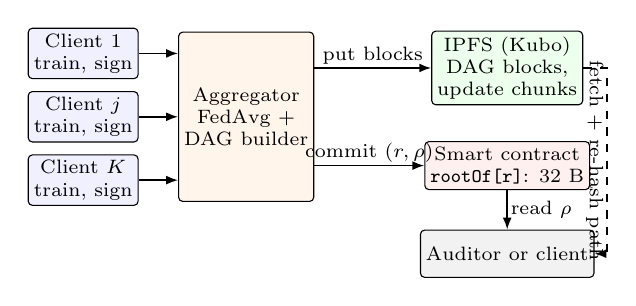
\begin{tikzpicture}[font=\scriptsize, node distance=4mm and 6mm,
  box/.style={draw, rounded corners=1.5pt, align=center, inner sep=2pt, minimum height=6mm},
  lab/.style={font=\scriptsize, inner sep=1pt},
  ar/.style={-{Latex[length=1.5mm]}, semithick}]
\node[box, fill=blue!6] (c1) {Client $1$\\ train, sign};
\node[box, fill=blue!6, below=1.5mm of c1] (c2) {Client $j$\\ train, sign};
\node[box, fill=blue!6, below=1.5mm of c2] (c3) {Client $K$\\ train, sign};
\node[box, fill=orange!8, right=5mm of c2, minimum width=1.55cm, minimum height=2.15cm] (agg) {Aggregator\\ FedAvg +\\ DAG builder};
\node[box, fill=green!7, minimum width=1.85cm] (ipfs) at ($(agg.east)+(2.45,0.62)$) {IPFS (Kubo)\\ DAG blocks,\\ update chunks};
\node[box, fill=red!6, minimum width=1.85cm] (sc) at ($(agg.east)+(2.45,-0.62)$) {Smart contract\\ \texttt{rootOf[r]}: 32 B};
\node[box, fill=gray!10, minimum width=1.85cm, below=5mm of sc] (aud) {Auditor or client};
\draw[ar] (c1.east) -- (c1.east -| agg.west); \draw[ar] (c2.east) -- (agg.west); \draw[ar] (c3.east) -- (c3.east -| agg.west);
\draw[ar] (agg.east |- ipfs.west) -- node[lab, above]{put blocks} (ipfs.west);
\draw[ar] (agg.east |- sc.west) -- node[lab, above]{commit $(r,\rho)$} (sc.west);
\draw[ar] (sc.south) -- node[lab, right]{read $\rho$} (aud.north);
\draw[ar, dashed] (ipfs.east) -- ++(3mm,0) |- node[lab, pos=0.25, sloped, below]{fetch + re-hash path} (aud.east);
\end{tikzpicture}
\caption{Recording and audit workflow. Only the 32-byte root digest $\rho$ goes on-chain; the inclusion path is content-addressed on IPFS and is available while it is pinned.}
\label{fig:arch}
\end{figure}

\begin{figure}[t]
\centering
\resizebox{\columnwidth}{!}{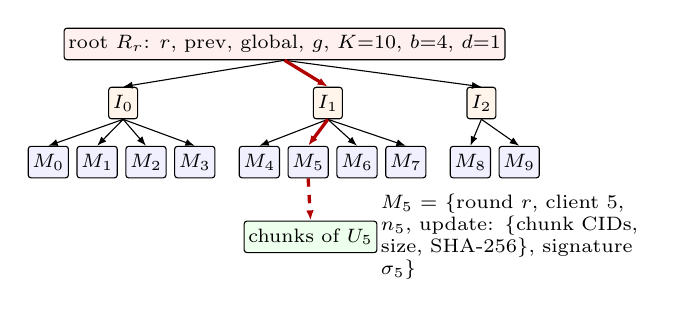
\begin{tikzpicture}[font=\scriptsize, x=1cm, y=1cm,
  nd/.style={draw, rounded corners=1pt, inner sep=1.5pt, align=center, minimum height=4mm},
  ar/.style={-{Latex[length=1.2mm]}}, hl/.style={-{Latex[length=1.3mm]}, very thick, red!70!black}]
\node[nd, fill=red!6] (root) at (3.1,1.5) {root $R_r$: $r$, prev, global, $g$, $K{=}10$, $b{=}4$, $d{=}1$};
\foreach \i/\x in {0/1.05,1/3.65,2/5.6}{\node[nd, fill=orange!8] (i\i) at (\x,0.75) {$I_{\i}$};}
\foreach \j in {0,...,9}{\pgfmathsetmacro{\xx}{0.1+0.62*\j+0.2*int(\j/4)}\node[nd, fill=blue!6, minimum width=4.6mm] (m\j) at (\xx,0) {$M_{\j}$};}
\draw[ar] (root.south) -- (i0.north); \draw[ar] (root.south) -- (i2.north); \draw[hl] (root.south) -- (i1.north);
\foreach \j in {0,1,2,3}{\draw[ar] (i0.south) -- (m\j.north);}
\foreach \j in {4,6,7}{\draw[ar] (i1.south) -- (m\j.north);}
\draw[hl] (i1.south) -- (m5.north);
\foreach \j in {8,9}{\draw[ar] (i2.south) -- (m\j.north);}
\node[nd, fill=green!7] (u5) at (3.43,-0.95) {chunks of $U_5$};
\draw[hl, dashed] (m5.south) -- (u5.north);
\node[align=left, text width=3.3cm, anchor=west, font=\scriptsize] at (4.2,-0.95) {$M_5$ = \{round $r$, client 5, $n_5$, update: \{chunk CIDs, size, SHA-256\}, signature $\sigma_5$\}};
\end{tikzpicture}}
\caption{Round DAG for $K=10$, $b=4$ (prev: root CID of round $r-1$; global: CID of the global-model node). Inner nodes and manifests are 0-indexed. The bold solid path (root, inner node, manifest) is the metadata inclusion path of client 5, whose size is reported as proof size; the dashed edge to the raw 256-KiB chunks of $U_5$ is an additional, separately costed fetch. Every block is fetched by CID and re-hashed.}
\label{fig:dag}
\end{figure}

\begin{table}[t]
\centering\scriptsize
\caption{DAG-CBOR block schema (canonical DAG-CBOR; map keys as encoded). CID: CIDv1 link with SHA2-256 (dag-cbor, or raw for chunks); integers are unsigned.}
\label{tab:schema}
\setlength{\tabcolsep}{3pt}
\begin{tabular}{@{}L{1.35cm}L{6.25cm}@{}}
\toprule
Block & Keys and values\\
\midrule
Root $R_r$ (its digest is on-chain) & \texttt{type}=\texttt{"fl-round"}, \texttt{v}=2, \texttt{round}=$r$, \texttt{k}=$K$, \texttt{fanout}=$b$, \texttt{depth}=$d$ (inner levels), \texttt{order}=\texttt{"client-id-asc"}, \texttt{children}: $\le b$ CIDs (inner nodes, or manifests if $d=0$), \texttt{prev}: CID of $R_{r-1}$ (null for $r=1$), \texttt{global}: CID of the model node, \texttt{ghash}: 32~B $g$\\
Inner $I$ & \texttt{type}=\texttt{"fl-inner"}, \texttt{children}: $\le b$ CIDs (next level or manifests)\\
Manifest $M_j$ & \texttt{type}=\texttt{"fl-client"}, \texttt{v}=2, \texttt{round}=$r$, \texttt{client}=$j$, \texttt{n}=$n_j$, \texttt{update}: \{\texttt{chunks}: raw CIDs of 256~KiB, \texttt{size}: bytes, \texttt{sha256}: 32~B, \texttt{enc}=\texttt{"f32le-sorted-keys"}\}, \texttt{sig}: 65~B ECDSA $(r,s,v)$ over the \texttt{FLC2} payload\\
Model node & \texttt{type}=\texttt{"fl-model"}, \texttt{round}=$r$, \texttt{blob}: descriptor as in \texttt{update}, \texttt{sha256}: $g$\\
\bottomrule
\end{tabular}
\end{table}

\subsection{Cost model and complexity}
S1a sends $K$ transactions, each writing a new 32-byte slot, and S1b writes $K$ slots in one call, so both grow linearly, $G_{\mathrm{S1}}(K)\approx \alpha K+\beta$ (marginal cost $\alpha$ per client, fixed part $\beta$), with $B_{\mathrm{S1a}}=132K$ (100~B calldata plus one 32-B slot per client) and $B_{\mathrm{S1b}}=100+64K$ on-chain bytes. S2, S2-sig and S3 send one call with a 32-byte root (68~B of calldata) and write one slot, so their gas and on-chain bytes are constant in $K$, with $B=100$~B. On-chain state grows $O(R)$ over $R$ rounds for the root registries and $O(RK)$ for S1. For an inclusion proof, S2 needs $\lceil\log_2K\rceil$ sibling hashes of 32~B plus a 4-B leaf index, held by an indexed proof service in our evaluation. S2-sig adds the 65-B signature, an 8-B $n_j$ and the 32-B global-model hash. The S3 metadata path is $d+2$ blocks, with $d=\max(0,\lceil\log_bK\rceil-1)$ inner levels (so $d=0$ when $K=1$ or when $b\ge K$): the root, $d$ inner nodes of at most $b$ links each, and the manifest. Counting only the child CID links is not enough, because the root and every inner node also carry non-link fields (Table~\ref{tab:schema}). A measurement with the same DAG-CBOR encoder (in-process store; no chain) gives a CID link of $c_\ell=\Nm{EqCidLinkB}$~B, a later-round root header of at most $h_R=\Nm{EqHeaderRootB}$~B (all non-children bytes, including \texttt{prev}, \texttt{global}, \texttt{ghash} and the CBOR headers; $h_R=\Nm{EqHeaderRootNullB}$~B when \texttt{prev} is null in round~1), and an inner-node header of at most $h_I=\Nm{EqHeaderInnerB}$~B. The path is therefore bounded by
\begin{equation}
P_{\mathrm{S3}}(K,b)\leq |M_j| + h_R + d\,h_I + c_\ell\,b\,(d+1).
\end{equation}
The manifest measures $|M_j|=\Nm{EqManFourKiBMin}$--\Nm{EqManFourKiBMax}$~B for a 4-KiB update (one chunk) and $\Nm{EqManPathsizeMin}$--\Nm{EqManPathsizeMax}$~B for a 424,356-B update (two chunks); the range is the CBOR integer width of the client identifier and of $n_j$. With these constants the bound held on every one of the \Nm{EqNpaths}{} measured paths (\Nm{EqNconfigs}{} configurations of $K$, $b$, update size and round, including a full root at $K=1000$, $b=4$). A flat root ($b=K$) has $P=O(K)$, while a fixed $b$ gives $O(|M|+b\log_b K)$. Minimising $b\log_b K$ alone would suggest $b=e$, but the per-block headers move the discrete minimum: among the fan-outs we measured, including $b=3$, the mean path at $K=1000$ was smallest at $b=\Nm{EqArgminB}$. Fig.~\ref{fig:proof}a does not include $b=3$; of the values it does show, $b=4$ is the smallest. The update chunks ($|U_j|$ bytes) are fetched in addition. Table~\ref{tab:complex} summarises the asymptotic costs of this implementation.

\begin{table}[t]
\centering\scriptsize
\caption{Asymptotic costs in $K$ and update size $|U|$, for this implementation (indexed S1/S2/S2-sig proofs). Proof size excludes the update itself. Building the round commitment is $O(K)$ for all schemes.}
\label{tab:complex}
\setlength{\tabcolsep}{2.2pt}
\begin{tabular}{@{}lcccc@{}}
\toprule
 & On-chain & Proof size & Verify one & Full audit\\
\midrule
S1 & $O(K)$ & $O(1)$ & $O(|U|)$ & $O(K|U|)$\\
S2, S2-sig & $O(1)$ & $O(\log K)$ & $O(\log K{+}|U|)$ & $O(K\log K{+}K|U|)$\\
S3 & $O(1)$ & $O(|M|{+}b\log_b K)$ & $O(b\log_b K{+}|U|)$ & $O(K\log_b K{+}K|U|)$\\
\bottomrule
\end{tabular}
\end{table}

\subsection{Verification and threat model}
Algorithm~\ref{alg:verify} is the auditor's check for a client with identifier $\mathit{id}$ at position $p$ in round $r$. Inner nodes are built bottom-up from consecutive groups of $b$, so only the right-most node of a level can be incomplete and earlier positions never shift; hence the child index is $\lfloor p/b^{\ell}\rfloor \bmod b$ on inner level $\ell<d$, $\lfloor p/b^{d}\rfloor$ at the root, and $p \bmod b$ in the last inner node (for a flat root, $d=0$ and $b=K$, it is $p$). If the auditor already knows the participant set, or receives $p$ from the client, $p$ is immediate. If only $\mathit{id}$ is known and participation may be partial, the auditor can locate $p$ by a binary search over the sorted manifests (inspecting an endpoint manifest under a child; $O(\log K)$ extra fetches on top of the inclusion path), or the root can carry an identifier list. Neither lookup is implemented or measured here: every reported run uses full participation, so $p=\mathit{id}$. Partial participation is supported by the ordering but is otherwise outside the evaluated scope. Every honest audit succeeded for all evaluated $K$ and $b$, including $K=10$, $b=4$ (Fig.~\ref{fig:dag}) and $K=1000$, $b=16$.

The aggregator is untrusted: it may alter, omit, substitute or replay records, including $n_j$. The IPFS provider may serve wrong bytes or withhold blocks. The chain is trusted for integrity and ordering. Clients generate and keep their keys and a receipt of their own update; auditors know each registered address $\mathcal{R}[j]$.

\begin{claim}\label{claim:int}
Assume SHA-256 is collision resistant, ECDSA is EUF-CMA secure, the chain returns the committed digest $\rho_r$, and the aggregator does not hold $sk_j$. If Algorithm~\ref{alg:verify} accepts identifier $\mathit{id}$ at position $p$ in round $r$, then the manifest, its $n_j$, the global-model hash $g$ and the update bytes $U_j$ it checked are those committed under $\rho_r$, and $(r,\mathit{id},n_j,\mathrm{SHA256}(U_j),g)$ was signed with the key registered as $\mathcal{R}[\mathit{id}]$.
\end{claim}
\emph{Proof sketch.} Each block is fetched by a CID that is either derived from $\rho_r$ or contained in an already verified block, and is accepted only if it hashes to that CID; serving a different block under the same CID requires a SHA-256 second preimage (and hence a collision). The claim assumes collision resistance, which implies second-preimage resistance, so by induction along the path every accepted block, and the chunk list, is the committed one. The manifest signature recovers to $\mathcal{R}[\mathit{id}]$ on a message that contains $r$, $\mathit{id}$, $n_j$, $\mathrm{SHA256}(U_j)$ and $g$; producing it for any altered tuple without $sk_j$ is an EUF-CMA forgery. A replay into another round changes $r$ and fails the signature or the contract guard. $\square$

What is \emph{not} guaranteed: (i)~omission of a client is detectable by that client, or by a third party that knows the expected participant set, but not by a third party who lacks that set; (ii)~the auditor does not re-compute FedAvg, so aggregation correctness beyond the bound $n_j$ and $g$ is out of scope; (iii)~availability is not guaranteed---a withheld block makes the check fail (T5); (iv)~if the aggregator holds client keys, Claim~\ref{claim:int} does not apply. In our experiments client keys were simulated in the aggregator process, so the tamper tests below exercise the verifier's checks, not a setting in which an adversarial aggregator lacks keys. A deployment must generate $sk_j$ on the client and distribute $\mathcal{R}$ without a per-round cost, e.g.\ as a DAG-CBOR address list committed once per federation epoch, or a registry contract paid once at enrolment; neither is implemented here. Integrity claims follow the transcript view of~\cite{rizzini}; poisoning and update privacy are out of scope.

\begin{algorithm}[t]
\caption{Per-client verification in S3}\label{alg:verify}
\small
\begin{algorithmic}[1]
\Require round $r$, identifier $\mathit{id}$, position $p$, registry $\mathcal{R}$
\State $c\gets \texttt{0x01711220}\,\Vert\,\texttt{rootOf}(r)$ \Comment{chain}
\State $N\gets\Call{Fetch}{c}$; check $N.\mathit{round}=r$, $p<N.k$
\State $g\gets N.\mathit{ghash}$; $b\gets N.\mathit{fanout}$; $d\gets N.\mathit{depth}$
\For{$\ell=d$ \textbf{down to} $1$}
\State $i\gets\lfloor p/b^{\ell}\rfloor$; \textbf{if} $\ell<d$ \textbf{then} $i\gets i \bmod b$
\State $N\gets\Call{Fetch}{N.\mathit{children}[i]}$
\EndFor
\State $M\gets\Call{Fetch}{N.\mathit{children}[p \bmod b]}$
\State check $M.\mathit{client}=\mathit{id}$, $M.\mathit{round}=r$; $h\gets M.\mathit{update}.\mathit{sha256}$
\State check $\mathrm{Recover}(M.\mathit{sig},(r,\mathit{id},M.n,h,g))=\mathcal{R}[\mathit{id}]$
\State fetch each chunk of $M.\mathit{update}$; check its CID
\State check $|U_{\mathit{id}}|=M.\mathit{update}.\mathit{size}$ and $\mathrm{SHA256}(U_{\mathit{id}})=h$
\State \Return accept \Comment{\textsc{Fetch} re-hashes every block}
\end{algorithmic}
\end{algorithm}

\subsection{S3 versus S2-sig proofs stored under one CID}\label{sec:residual}
An S2-sig aggregator could also write each client's proof object (siblings, leaf index, $\sigma_j$, $n_j$, $g$) to IPFS. S3 adds no cryptographic guarantee over that design: both rest on SHA-256 and on the client signature (Claim~\ref{claim:int}). The difference lies in what the chain commits to. (i)~If the chain stores only the Merkle root, the proof objects are not bound to the commitment; the auditor must learn where they are from the aggregator. Committing their CID as well would add a second 32-byte slot in the storage variant, or 32 more bytes of calldata and log data in the event-only variant already measured for a single root (164~B, Table~\ref{tab:cost}); we did not implement this two-value alternative. (ii)~If the chain stores only the CID of a proof bundle, the bundle must be split per client to keep one audit small, and must record $r$, $K$, the ordering rule and the global model so that a position can be resolved; that bundle is then a hash-linked DAG of the kind S3 specifies, and the separate Merkle root becomes redundant. In S3 the commitment and the inclusion path are the same object: the on-chain digest is the root CID, the path blocks are the proof, and the root carries $r$, $K$, $b$, $d$, \texttt{prev} and the global-model reference. The remaining advantage is discoverability: one 32-byte value lets an auditor locate every path from the commitment (enumerating all $K$ manifests still costs $O(K)$ fetches). Availability still depends on pinning, as it would for an S2-sig bundle. We therefore claim this self-describing packaging and its measured costs, not a stronger integrity property than S2-sig.

\section{Experimental setup}\label{sec:setup}
\textbf{Platform.} All runs used one virtual machine. \texttt{lscpu} reports a KVM guest with the model string ``Intel(R) Xeon(R) Processor'' (family 6, model 207, stepping 2) and no SKU; we do not infer one. It has 8 vCPUs (one thread per core), 16~GiB RAM and no swap; storage is a virtio block device whose backing medium is not exposed to the guest, and no CPU-frequency governor is visible. Software: Debian 13.7, Linux 6.12, Python 3.13.5, PyTorch 2.14.1 on CPU, a local Anvil v1.9.0 chain (id 31337, Prague; non-local RPCs are refused, no real funds), Solidity 0.8.28 and Kubo 0.43.1. Anvil, Kubo and the Python recorder ran co-located on this guest; processes were not pinned to CPUs. For the grid and the clean run, one offline Kubo daemon on the same guest served all blocks, so Table~\ref{tab:time} verification times are local block reads, not peer-to-peer fetches; its \texttt{dag/put} reproduces our locally computed CIDs. Peer-to-peer retrieval is measured separately (Section~\ref{sec:ipfs}).

\textbf{FL workload.} We use PneumoniaMNIST (2 classes, 4,708 training images) and PathMNIST (9 classes, 89,996) at $28\times28$ from MedMNIST+ v3.0~\cite{medmnist,medmnistplus} with the official splits. A small CNN (105,346 parameters for one input channel, 106,089 for three; 421,384 and 424,356~B per update) is trained for one local epoch per round (Adam, learning rate $10^{-3}$, batch 64). FedAvg runs 20 rounds with full participation in an in-repository loop; a three-round diagnostic on one setting produced the same losses as Flower 1.43~\cite{flower}, but the grid itself did not invoke Flower. The grid covers $K\in\{10,50,100\}$, IID and Dirichlet partitions with $\alpha\in\{0.1,0.5\}$~\cite{hsu} and 3 seeds (54 runs). A Dirichlet draw required at least 10 samples per client, relaxed to 5 and then 2 after 1,000 and 10,000 further draws. PneumoniaMNIST with $\alpha=0.5$, $K=100$ needed the minimum of 2; with $\alpha=0.1$, $K\in\{50,100\}$ no feasible partition was found in 21,000 draws, so these 6 runs are N/A and 48 completed. Accuracy does not affect gas, bytes or proof size; the grid was not rerun.


\textbf{Schemes and metrics.} Every round is recorded under all schemes from the same updates: \Sa, \Sb, S2 (binary SHA-256 Merkle tree~\cite{merkle}), S2-sig and S3 with $b\in\{\text{flat},16,4\}$, each in a storage and an event-only variant. The S1 contract used for the gas table has no round guard, so that those gas figures remain comparable to the earlier measurements; a guarded S1 variant is used only in T4. Gas and on-chain bytes (calldata, new slots, log bytes) come from receipts of rounds $\geq2$, since round~1 also initialises \texttt{lastRound}, and are taken from the FedAvg grid at $K\le100$ and from a synthetic cost test at $K\ge500$ (3 rounds, so 2 rounds $\geq2$, with 4-KiB updates). The reported local RPC times and verification times come from a separate clean run without training (synthetic 424,356-B updates of the PathMNIST model size, $K\in\{10,50,100,500,1000\}$, 10 rounds; all clients audited for $K\le100$, 200 random clients per round otherwise). S1/S2/S2-sig verifiers perform a per-client index lookup rather than loading an $O(K)$ bundle. Tamper tests T1--T6 were repeated on a dedicated campaign of \Nm{TamperRuns}{} two-round recordings (the same $K$-mix as the 48 completed grid runs plus the five synthetic sizes, with 4-KiB updates). Grid timings are not used; local RPC times exclude public-network block time and confirmation.

\textbf{Two-peer DAG-path test.} To test retrieval of the actual round path rather than of random blocks, we ran three private Kubo daemons on the same guest (loopback, empty bootstrap, mDNS off, no public network): provider $A$ (the aggregator), an initially empty auditor peer $B$, and a replica peer $C$. For $K\in\{100,1000\}$ and $b\in\{16,4\}$, $A$ stored \Nm{DagSizeB}-B synthetic updates signed with fresh keys, built one round DAG per fan-out, pinned each root recursively and committed its digest to a local registry contract. For \Nm{DagNaudKonehundred}{} clients ($K=100$: all) or \Nm{DagNaudKonethousand}{} random clients ($K=1000$), $B$ read \texttt{rootOf}(1) from the chain and ran Algorithm~\ref{alg:verify} over bitswap, first for the metadata path only and then with the update chunks; $B$ deleted fetched blocks after every trial (cold fetches). For T5, $C$ pinned the $b=16$ root recursively and was then stopped; $A$ unpinned the roots and deleted, for \Nm{WhN}{} random clients, either the manifest or one update chunk. $B$ then retried those clients with $C$ offline (\Nm{DagTimeout}-s block timeout) and again after $C$ was restarted.

\section{Results}\label{sec:results}
\begin{table*}[t]
\centering\footnotesize
\caption{On-chain cost per round (median of rounds $\geq2$). Storage variant except the two event columns. $K\le100$: FedAvg grid; $K\ge500$: the two synthetic rounds (their $\Delta$ values are reported in the text). $\Delta$ = S3 $-$ S2.}
\label{tab:cost}
\setlength{\tabcolsep}{4.5pt}
\begin{tabular}{@{}r rrrrr rr rrr@{}}
\toprule
 & \multicolumn{5}{c}{Gas per round, storage} & \multicolumn{2}{c}{Gas, event} & \multicolumn{3}{c}{On-chain bytes, storage}\\
\cmidrule(lr){2-6}\cmidrule(lr){7-8}\cmidrule(l){9-11}
$K$ & S1a & S1b & S2 & S3 ($b$=16) & $\Delta$ & S2 & S3 & S1a & S1b & S2, S3\\
\midrule
10   & \Nm{GasSoneaK10} & \Nm{GasSonebK10} & \Nm{GasStwoK10} & \Nm{GasSthreeK10} & \Nm{GasGapK10} & \Nm{GasEventStwoK10} & \Nm{GasEventSthreeK10} & \Nm{BytesSoneaK10} & \Nm{BytesSonebK10} & 100\\
50   & \Nm{GasSoneaK50} & \Nm{GasSonebK50} & \Nm{GasStwoK50} & \Nm{GasSthreeK50} & \Nm{GasGapK50} & \Nm{GasEventStwoK50} & \Nm{GasEventSthreeK50} & \Nm{BytesSoneaK50} & \Nm{BytesSonebK50} & 100\\
100  & \Nm{GasSoneaK100} & \Nm{GasSonebK100} & \Nm{GasStwoK100} & \Nm{GasSthreeK100} & \Nm{GasGapK100} & \Nm{GasEventStwoK100} & \Nm{GasEventSthreeK100} & \Nm{BytesSoneaK100} & \Nm{BytesSonebK100} & 100\\
500  & \Nm{GasSoneaK500} & \Nm{GasSonebK500} & \Nm{GasStwoK500} & \Nm{GasSthreeK500} & \Nm{GasGapK500} & \Nm{GasEventStwoK500} & \Nm{GasEventSthreeK500} & \Nm{BytesSoneaK500} & \Nm{BytesSonebK500} & 100\\
1000 & \Nm{GasSoneaK1000} & \Nm{GasSonebK1000} & \Nm{GasStwoK1000} & \Nm{GasSthreeK1000} & \Nm{GasGapK1000} & \Nm{GasEventStwoK1000} & \Nm{GasEventSthreeK1000} & \Nm{BytesSoneaK1000} & \Nm{BytesSonebK1000} & 100\\
\bottomrule
\end{tabular}
\end{table*}

\begin{table*}[t]
\centering\footnotesize
\caption{Clean timing run (424,356-B updates, 10 rounds; medians, verify with IQR). ``S3 total'' adds building and storing the DAG ($b=16$). Verify checks one client, including reading its update from the local Kubo daemon; S1/S2/S2-sig use indexed lookups.}
\label{tab:time}
\setlength{\tabcolsep}{4.2pt}
\begin{tabular}{@{}r rrrrr cccc@{}}
\toprule
 & \multicolumn{5}{c}{Local RPC time (ms)} & \multicolumn{4}{c}{Per-client verify, median [IQR] (ms)}\\
\cmidrule(lr){2-6}\cmidrule(l){7-10}
$K$ & S1a & S1b & S2 & S3 & S3 total & S1 & S2 & S2-sig & S3 ($b$=16)\\
\midrule
10 & \Nm{TchainSoneaK10} & \Nm{TchainSonebK10} & \Nm{TchainStwoK10} & \Nm{TchainSthreeK10} & \Nm{TtotalSthreeK10} & \Nm{TverSoneK10} [\Nm{TverSoneK10Qone}--\Nm{TverSoneK10Qthree}] & \Nm{TverStwoK10} [\Nm{TverStwoK10Qone}--\Nm{TverStwoK10Qthree}] & \Nm{TverStwosigK10} [\Nm{TverStwosigK10Qone}--\Nm{TverStwosigK10Qthree}] & \Nm{TverSthreeK10} [\Nm{TverSthreeK10Qone}--\Nm{TverSthreeK10Qthree}]\\
50 & \Nm{TchainSoneaK50} & \Nm{TchainSonebK50} & \Nm{TchainStwoK50} & \Nm{TchainSthreeK50} & \Nm{TtotalSthreeK50} & \Nm{TverSoneK50} [\Nm{TverSoneK50Qone}--\Nm{TverSoneK50Qthree}] & \Nm{TverStwoK50} [\Nm{TverStwoK50Qone}--\Nm{TverStwoK50Qthree}] & \Nm{TverStwosigK50} [\Nm{TverStwosigK50Qone}--\Nm{TverStwosigK50Qthree}] & \Nm{TverSthreeK50} [\Nm{TverSthreeK50Qone}--\Nm{TverSthreeK50Qthree}]\\
100 & \Nm{TchainSoneaK100} & \Nm{TchainSonebK100} & \Nm{TchainStwoK100} & \Nm{TchainSthreeK100} & \Nm{TtotalSthreeK100} & \Nm{TverSoneK100} [\Nm{TverSoneK100Qone}--\Nm{TverSoneK100Qthree}] & \Nm{TverStwoK100} [\Nm{TverStwoK100Qone}--\Nm{TverStwoK100Qthree}] & \Nm{TverStwosigK100} [\Nm{TverStwosigK100Qone}--\Nm{TverStwosigK100Qthree}] & \Nm{TverSthreeK100} [\Nm{TverSthreeK100Qone}--\Nm{TverSthreeK100Qthree}]\\
500 & \Nm{TchainSoneaK500} & \Nm{TchainSonebK500} & \Nm{TchainStwoK500} & \Nm{TchainSthreeK500} & \Nm{TtotalSthreeK500} & \Nm{TverSoneK500} [\Nm{TverSoneK500Qone}--\Nm{TverSoneK500Qthree}] & \Nm{TverStwoK500} [\Nm{TverStwoK500Qone}--\Nm{TverStwoK500Qthree}] & \Nm{TverStwosigK500} [\Nm{TverStwosigK500Qone}--\Nm{TverStwosigK500Qthree}] & \Nm{TverSthreeK500} [\Nm{TverSthreeK500Qone}--\Nm{TverSthreeK500Qthree}]\\
1000 & \Nm{TchainSoneaK1000} & \Nm{TchainSonebK1000} & \Nm{TchainStwoK1000} & \Nm{TchainSthreeK1000} & \Nm{TtotalSthreeK1000} & \Nm{TverSoneK1000} [\Nm{TverSoneK1000Qone}--\Nm{TverSoneK1000Qthree}] & \Nm{TverStwoK1000} [\Nm{TverStwoK1000Qone}--\Nm{TverStwoK1000Qthree}] & \Nm{TverStwosigK1000} [\Nm{TverStwosigK1000Qone}--\Nm{TverStwosigK1000Qthree}] & \Nm{TverSthreeK1000} [\Nm{TverSthreeK1000Qone}--\Nm{TverSthreeK1000Qthree}]\\
\bottomrule
\end{tabular}
\end{table*}


\textbf{On-chain cost.} Table~\ref{tab:cost} shows the central cost result; the S3 medians are identical for $b\in\{\text{flat},16,4\}$. Over all grid and synthetic runs, the storage variant costs \Nm{GasStwoMin}--\Nm{GasStwoMax}{} gas for S2 and \Nm{GasSthreeMin}--\Nm{GasSthreeMax}{} gas for S3 at every fan-out, always with 100 on-chain bytes; the event variant costs \Nm{GasEventStwoMin}--\Nm{GasEventStwoMax}{} gas for S2 and \Nm{GasEventSthreeMin}--\Nm{GasEventSthreeMax}{} gas for S3, always with 164~B (68~B calldata plus 96~B of log topics and data). The median S3$-$S2 difference is \Nm{GasGapMedMin}--\Nm{GasGapMedMax}{} gas (Table~\ref{tab:cost}). In all \Nm{GasGapPairs}{} paired rounds it equals a fixed 22 gas plus 12 gas per extra non-zero byte in the 32-byte root (16 gas per non-zero and 4 per zero calldata byte), so per-round differences range from \Nm{GasGapRoundMin}{} to \Nm{GasGapRoundMax}{} gas. At $K=500$ the two rounds differ by \Nm{GasGapK500Rtwo}{} and \Nm{GasGapK500Rthree}{} gas (median 16); at $K=1000$ both rounds differ by \Nm{GasGapK1000Rtwo}{} gas. S2-sig writes the same 32-byte root as S2: in the clean timing run (\Nm{GasSigPairsClean}{} paired storage rounds $\geq2$) and the tamper campaign (\Nm{GasSigPairsTamper}{}), the S2-sig$-$S2 gas difference ranges from \Nm{GasSigGapMin}{} to \Nm{GasSigGapMax}{} gas (median \Nm{GasSigGapMed}), consistent with calldata byte values only. A linear fit gives $\alpha=\Nm{FitSoneaSlope}$ (S1a) and $\Nm{FitSonebSlope}$ (S1b) gas per client in the storage variant ($\beta=\Nm{FitSoneaIntercept}$ and $\Nm{FitSonebIntercept}$) and $\Nm{FitSoneaEventSlope}$ and $\Nm{FitSonebEventSlope}$ in the event variant. In round~1, S2 and S3 cost \Nm{GasStwoRoundOne}{} and \Nm{GasSthreeRoundOne}{} gas because the round counter is first written. The event variant is about 40\% cheaper but depends on log retention, which matters for a long audit window if a client or node prunes history; the storage variant lets auditors read $\texttt{rootOf}(r)$ from state. Under current Ethereum mainnet rules (Fusaka/Osaka, 3 December 2025, UTC), EIP-7825 caps a single transaction at $2^{24}=16{,}777{,}216$ gas, so an S1b storage transaction would have to be split above about $K=\Nm{EipSonebKcap}$ (at $K=1000$ the measured S1b gas is \Nm{GasSonebK1000}). S2, S2-sig and S3 remain far below that cap. These gas figures are execution costs on a local Prague chain; on a rollup they would be dominated by layer-1 data posting, which we do not measure.

\begin{figure}[t]
\centering
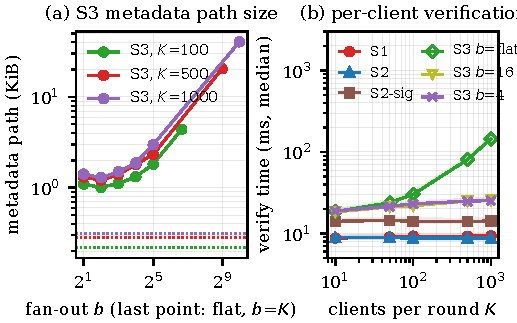
\includegraphics[width=\columnwidth]{figs/fig4_proof_verify.pdf}
\caption{(a) Mean S3 metadata-path size versus fan-out (4-KiB updates; root, inner nodes and manifest, without update chunks); dotted lines show the S2 Merkle path (including the 4-B index) for the same $K$. (b) Median per-client verification time from the clean timing run, with IQR bands; S1/S2/S2-sig use indexed lookups.}
\label{fig:proof}
\end{figure}

\textbf{Proof size and verification.} Fig.~\ref{fig:proof}a confirms the fan-out trade-off. At $K=1000$ with 4-KiB updates the mean S3 metadata path is \Nm{PszSthreeK1000}~B ($b=16$) and \Nm{PszSthreeFourK1000}~B ($b=4$), against \Nm{PszSthreeFlatK1000}~B for a flat root and a mean S2 path of \Nm{PszStwoK1000}~B (max \Nm{PszStwoK1000Max}~B). The 4-B index plus $\lceil\log_2 1000\rceil=10$ siblings would be 324~B; the slightly smaller mean is due to odd-node promotion in the Merkle tree, which shortens the path of some leaves. In the clean run with 424,356-B updates, the corresponding S3 metadata paths are \Nm{ProofSthreeK1000}~B, \Nm{ProofSthreeFourK1000}~B and \Nm{ProofSthreeFlatK1000}~B, with \Nm{NfetchSthreeK1000}{} and \Nm{NfetchSthreeFourK1000}{} fetched metadata blocks; the update chunks add $|U_j|$. These clean-run paths are a few tens of bytes larger than the Table~\ref{tab:ipfs} means (\Nm{DagPathKonethousandBsixteen}~B and \Nm{DagPathKonethousandBfour}~B) because that test uses round~1, whose root has a null \texttt{prev}, whereas the clean run includes later rounds whose root carries a previous-round CID. S3 paths are larger than the S2 path because they carry the signed manifest and chunk list. With an indexed proof service, median verification of S1, S2 and S2-sig stays nearly flat from $K=10$ to 1000 (Table~\ref{tab:time}, Fig.~\ref{fig:proof}b). S3 with $b=16$ rises from \Nm{TverSthreeK10} to \Nm{TverSthreeK1000}~ms, consistent with $b\log_b K$, and from \Nm{TverSthreeFourK10} to \Nm{TverSthreeFourK1000}~ms with $b=4$; a flat root reaches \Nm{TverSthreeFlatK1000}~ms. S3 is thus not faster than an indexed lookup. All honest verifications succeeded; times include reading $U_j$ and thus scale with model size.

\textbf{Recording latency.} The local RPC time of S2 and S3 stays at \Nm{TchainStwoSthreeMin}--\Nm{TchainStwoSthreeMax}~ms for all $K$, while S1a grows with its $K$ transactions (Table~\ref{tab:time}). S3 pays off-chain: building and storing the DAG raises its total to \Nm{TtotalSthreeK1000}~ms at $K=1000$ ($b=16$), of which the median DAG construction (encoding and metadata \texttt{block/put}) is \Nm{TbuildSthreeK1000}~ms; we do not have a separate encode-versus-put split and did not evaluate a single CAR import. The S2 total of \Nm{TtotalStwoK1000}~ms on the same clean run is tree construction (\Nm{TbuildStwoK1000}~ms) plus the \Nm{TchainStwoK1000}~ms local RPC in Table~\ref{tab:time}. Storing the update blobs, common to all schemes, took \Nm{TblobK100}~ms at $K=100$ and \Nm{TblobK1000}~ms at $K=1000$.

\begin{table}[t]
\centering\scriptsize
\caption{Tamper tests: runs detected out of \Nm{TamperRuns}{}. n/t: not applicable (the scheme does not bind that field). T4 is compared only among contracts that enforce $r=\texttt{lastRound}+1$.}
\label{tab:tamper}
\setlength{\tabcolsep}{2.0pt}
\begin{tabular}{@{}p{0.48cm}p{3.55cm}cccc@{}}
\toprule
Test & Manipulation & S1 & S2 & S2-sig & S3\\
\midrule
T1 & one byte of a stored client update flipped & \Nm{TamperT1S1} & \Nm{TamperT1S2} & \Nm{TamperT1S2sig} & \Nm{TamperT1S3}\\
T2 & client record replaced by a forged update & \Nm{TamperT2S1} & \Nm{TamperT2S2} & \Nm{TamperT2S2sig} & \Nm{TamperT2S3}\\
T3a & aggregator omits a client; the client checks its receipt & \Nm{TamperT3aS1} & \Nm{TamperT3aS2} & \Nm{TamperT3aS2sig} & \Nm{TamperT3aS3}\\
T3b & substitute signed with an unregistered key & n/t & \Nm{TamperT3bS2} & \Nm{TamperT3bS2sig} & \Nm{TamperT3bS3}\\
T4 & re-commit of round~1 on a guarded registry & \Nm{TamperT4S1guard} & \Nm{TamperT4S2} & \Nm{TamperT4S2sig} & \Nm{TamperT4S3}\\
T5 & data withheld (blob, proof store or manifest) & \Nm{TamperT5S1} & \Nm{TamperT5S2} & \Nm{TamperT5S2sig} & \Nm{TamperT5S3}\\
T6 & only $n_j$ changed, original signature kept & n/t & n/t & \Nm{TamperT6S2sig} & \Nm{TamperT6S3}\\
\bottomrule
\end{tabular}
\end{table}

\textbf{Tamper tests.} Table~\ref{tab:tamper} reports detection counts (outcomes are deterministic given the implementation). T1, T2, T3a and T5 were detected by every applicable scheme. T3b and T6 were detected by S3 and by S2-sig, because the signature does not recover to the registered address or does not cover the altered $n_j$. An unsigned S2 leaf has no signature, so the T3b forgery verified, and T6 is not applicable to S1 or S2, which do not bind $n_j$. T4 reverted on every guarded registry, including a guarded S1 variant; it is a contract property, not a property of the commitment. S1 has no attribution check (T3b n/t). Because client keys were simulated in the aggregator process, these tests do not model an aggregator that holds client keys (Claim~\ref{claim:int}, (iv)).


\begin{table}[t]
\centering\scriptsize
\caption{Two-peer DAG-path test on one machine (three private Kubo daemons, loopback, no public network). Cold fetches by auditor peer $B$ from provider $A$, including the chain read and all checks of Algorithm~\ref{alg:verify}; medians with IQR in brackets (ms); all \Nm{DagOkAll}{} trials verified. Blocks: metadata blocks per path; Path: mean metadata-path size.}
\label{tab:ipfs}
\setlength{\tabcolsep}{2.4pt}
\begin{tabular}{@{}rrrrcc@{}}
\toprule
$K$ & $b$ & Blocks & Path (B) & Metadata only & With update\\
\midrule
100 & 16 & \Nm{DagBlocksKonehundredBsixteen} & \Nm{DagPathKonehundredBsixteen} & \Nm{DagMetaMedKonehundredBsixteen} [\Nm{DagMetaQoneKonehundredBsixteen}--\Nm{DagMetaQthreeKonehundredBsixteen}] & \Nm{DagFullMedKonehundredBsixteen} [\Nm{DagFullQoneKonehundredBsixteen}--\Nm{DagFullQthreeKonehundredBsixteen}]\\
100 & 4 & \Nm{DagBlocksKonehundredBfour} & \Nm{DagPathKonehundredBfour} & \Nm{DagMetaMedKonehundredBfour} [\Nm{DagMetaQoneKonehundredBfour}--\Nm{DagMetaQthreeKonehundredBfour}] & \Nm{DagFullMedKonehundredBfour} [\Nm{DagFullQoneKonehundredBfour}--\Nm{DagFullQthreeKonehundredBfour}]\\
1000 & 16 & \Nm{DagBlocksKonethousandBsixteen} & \Nm{DagPathKonethousandBsixteen} & \Nm{DagMetaMedKonethousandBsixteen} [\Nm{DagMetaQoneKonethousandBsixteen}--\Nm{DagMetaQthreeKonethousandBsixteen}] & \Nm{DagFullMedKonethousandBsixteen} [\Nm{DagFullQoneKonethousandBsixteen}--\Nm{DagFullQthreeKonethousandBsixteen}]\\
1000 & 4 & \Nm{DagBlocksKonethousandBfour} & \Nm{DagPathKonethousandBfour} & \Nm{DagMetaMedKonethousandBfour} [\Nm{DagMetaQoneKonethousandBfour}--\Nm{DagMetaQthreeKonethousandBfour}] & \Nm{DagFullMedKonethousandBfour} [\Nm{DagFullQoneKonethousandBfour}--\Nm{DagFullQthreeKonethousandBfour}]\\
\midrule
\multicolumn{6}{@{}l@{}}{T5, $b=16$: \Nm{WhN}{} clients; $A$ unpinned and deleted the}\\
\multicolumn{6}{@{}l@{}}{manifest (10 clients) or one update chunk (10 clients).}\\
\multicolumn{6}{@{}l@{}}{\quad Replica $C$ offline: detected \Nm{WhOffDetKonehundred} ($K=100$), \Nm{WhOffDetKonethousand} ($K=1000$)}\\
\multicolumn{6}{@{}l@{}}{\quad Replica $C$ online: verified \Nm{WhOnOkKonehundred} (\Nm{WhOnMedKonehundred}~ms), \Nm{WhOnOkKonethousand} (\Nm{WhOnMedKonethousand}~ms)}\\
\bottomrule
\end{tabular}
\end{table}

\textbf{Two-peer DAG-path retrieval.}\label{sec:ipfs} Table~\ref{tab:ipfs} reports the new test. Starting from the on-chain digest, auditor peer $B$ fetched and verified the committed path of every sampled client from provider $A$ (\Nm{DagOkAll}{} trials). The cold metadata path took a median of \Nm{DagMetaMedKonehundredBsixteen}~ms ($K=100$, $b=16$) to \Nm{DagMetaMedKonethousandBfour}~ms ($K=1000$, $b=4$), and the full path with the 424,356-B update \Nm{DagFullMedKonehundredBsixteen}--\Nm{DagFullMedKonethousandBfour}~ms. Smaller fan-outs need more blocks, hence more bitswap round trips. Pinning the whole round on $A$ took \Nm{DagPinAKonethousandBsixteen}~ms at $K=1000$ ($b=16$), and the replica pin on $C$ took \Nm{WhRepPinKonehundred}~s ($K=100$) and \Nm{WhRepPinKonethousand}~s ($K=1000$, \Nm{WhRepMiBKonethousand}~MiB). Those pin times are local disk and loopback figures, not the transfer times a remote replica would see. When $A$ withheld a manifest or a chunk and $C$ was offline, every audit of those clients failed at the block timeout, i.e.\ T5 was detected but not repaired; once $C$ was online, all of them verified without any change to the chain. A deployment should retry a missing block and treat a persistent timeout as detection, not as a unique diagnosis of withholding versus slow discovery; we used a single \Nm{DagTimeout}~s timeout in this same-machine test. These times bound software overhead only, not wide-area or DHT delays. The metadata DAG of one such round (root, inner nodes and all manifests, without update chunks) was \Nm{DagMetaBKonethousandBsixteen}~B at $b=16$ and \Nm{DagMetaBKonethousandBfour}~B at $b=4$, against the \Nm{WhRepMiBKonethousand}~MiB full replica pin that includes every update chunk.

\textbf{FedAvg sanity check.} PathMNIST test accuracy (mean $\pm$ s.d., 3 seeds, round 20) fell from $0.770\pm0.006$ (IID, $K=10$) to $0.447\pm0.061$ (Dirichlet $\alpha=0.1$, $K=100$); PneumoniaMNIST reached $0.850\pm0.014$ (IID, $K=10$), but \Nm{AccPneuFloorCells}{} of the \Nm{AccPneuCells}{} completed PneumoniaMNIST cells (\Nm{AccPneuFloorRuns}{} of \Nm{AccCompletedRuns}{} completed runs) stayed at $0.625\pm0.000$, likely a majority-class floor. Our claim concerns auditability, not model quality.


\section{Discussion and limitations}\label{sec:disc}
S3 matches the on-chain cost of a Merkle root and moves custody of the inclusion path from the aggregator to content-addressed storage, but only while blocks stay pinned. In our test the aggregator pinned each committed root recursively from commit until it deliberately unpinned it for T5, and a replica peer pinned the $b=16$ root; the whole run lasted \Nm{DagWallMin}~min, so this shows the roles, not a retention period. The test shows that withholding is detected, not repaired, and that a second peer can fetch a withheld block only if another custodian pins it. Custody of metadata and of update chunks can be split. An auditor or a consortium can pin only the metadata DAG (\Nm{DagMetaBKonethousandBsixteen}~B per round at $K=1000$, $b=16$; \Nm{DagMetaBKonethousandBfour}~B at $b=4$), while each client pins its own chunks. If only the metadata is replicated, an auditor can still check signatures, $n_j$, $g$ and the committed chunk digests, but cannot re-hash the update bytes unless those chunks are pinned elsewhere. A full replica that holds every chunk, as $C$ did in the test, stored \Nm{WhRepMiBKonethousand}~MiB for one $K=1000$ round. A deployment should therefore name its custodians: the aggregator for the audit window, plus at least one independent metadata pinner, and clients (or another store) for update chunks; the retention period is a policy choice that we did not measure. ``Anyone can fetch the path'' is thus a property of content addressing plus pinning, supported here by a same-machine sanity test, not a wide-area measurement: all peers shared one guest, kernel and disk, and DHT discovery, NAT traversal, wide-area delay and public-gateway retrieval were not exercised. Updates are unencrypted, which does not suit a clinical deployment (ciphertext chunks would still have CIDs, but are not evaluated); client keys were simulated in the aggregator; gas is exact for Prague rules, subject to EIP-7825; poisoning is out of scope. Six PneumoniaMNIST Dirichlet cells ($\alpha=0.1$, $K\in\{50,100\}$) were infeasible and are reported as N/A, not estimated.

\section{Conclusion}\label{sec:concl}
Writing only the 32-byte digest of a hierarchical CID per FL round kept the on-chain cost at \Nm{GasSthreeMin}--\Nm{GasSthreeMax}{} gas and 100 bytes from 10 to 1000 clients, matching a Merkle-root baseline up to calldata byte values (median difference \Nm{GasGapMedMin}--\Nm{GasGapMedMax}{} gas). With signatures that bind $n_j$ and the global-model hash, S3 and a signed-leaf Merkle root both detect an unregistered substitute and an isolated weight change that an unsigned leaf misses. A fan-out of 16 or 4 keeps the metadata path at about 2~KiB at 1000 clients (\Nm{ProofSthreeK1000}~B in the clean run at $b=16$; \Nm{DagPathKonethousandBsixteen}~B in the round-1 DAG-path test), with the update fetched in addition. With an indexed proof service, S3 is not faster to verify than S1 or S2; its remaining distinction is packaging: the signed inclusion path is the content-addressed DAG under the committed root, which a second IPFS peer fetched and verified in a same-machine test. The main costs are off-chain DAG construction and the need for reliable, replicated pinning. Future work will evaluate retrieval across distinct hosts, client-held keys and encrypted updates.
\label{bodyend}

\section*{CRediT authorship contribution statement}
\textbf{Prayitno:} Conceptualization, Methodology, Software, Investigation, Writing -- original draft. \textbf{Karisma Trinanda Putra:} Conceptualization, Supervision, Validation, Funding acquisition, Writing -- review \& editing. \textbf{Cahya Damarjati:} Methodology, Validation. \textbf{Sunardi:} Formal analysis, Visualization. \textbf{Wiktasari:} Software, Data curation. \textbf{Suko Tyas Pernanda:} Software, Investigation. \textbf{Liliek Triyono:} Validation, Writing -- review \& editing.

\section*{Declaration of competing interest}
The authors declare that they have no known competing financial interests or personal relationships that could have appeared to influence the work reported in this paper.

\section*{Funding}
This work was supported by the Research Fellowship programme of Universitas Muhammadiyah Yogyakarta, which has no grant number. The funder had no role in the study design, analysis, writing or the decision to submit.

\section*{Data availability}
The study uses only the public MedMNIST+ v3.0 dataset (PneumoniaMNIST and PathMNIST, CC BY 4.0)~\cite{medmnistplus}; no ethical approval was required. The code, contracts and result files that reproduce the tables and figures are available at \href{https://github.com/kang-prayit/fl-onchain-hcid}{github.com/\mbox{kang-prayit}/\mbox{fl-onchain-hcid}}.

\section*{Declaration of generative AI and AI-assisted technologies in the manuscript preparation process}
During the preparation of this work the authors used an AI-assisted writing tool in order to draft and edit the manuscript text. After using this tool, the authors reviewed and edited the content as needed and take full responsibility for the content of the published article. All figures were produced from matplotlib and TikZ code; no generative AI was used to create or alter figures.

\setlength{\bibsep}{0pt plus 0.3pt}
\renewcommand{\bibfont}{\footnotesize}
\begin{thebibliography}{27}
\bibitem{kairouz} P. Kairouz, H.B. McMahan, et al., Advances and open problems in federated learning, Found. Trends Mach. Learn. 14 (1--2) (2021) 1--210. \url{https://doi.org/10.1561/2200000083}.

\bibitem{mcmahan} H.B. McMahan, E. Moore, D. Ramage, S. Hampson, B. Ag\"uera y Arcas, Communication-efficient learning of deep networks from decentralized data, in: Proc. 20th Int. Conf. Artif. Intell. Stat. (AISTATS), PMLR 54 (2017) 1273--1282. \url{https://proceedings.mlr.press/v54/mcmahan17a.html}.

\bibitem{prayitno2021} Prayitno, C.-R. Shyu, K.T. Putra, H.-C. Chen, Y.-Y. Tsai, K.S.M.T. Hossain, W. Jiang, Z.-Y. Shae, A systematic review of federated learning in the healthcare area: From the perspective of data properties and applications, Appl. Sci. 11 (23) (2021) 11191. \url{https://doi.org/10.3390/app112311191}.

\bibitem{pamungkas2026} Y. Pamungkas, Y. Thwe, M.M. Aung, A. Karim, Collaborative intelligence in oncology: A review of federated learning models for cancer detection, J. Robot. Control 7 (2) (2026) 3489--3501. \url{https://doi.org/10.18196/jrc.v7i2.28497}.

\bibitem{putra2024iomt} K.T. Putra, A.Z. Arrayyan, N. Hayati, Firdaus, C. Damarjati, A. Bakar, H.-C. Chen, A review on the application of Internet of Medical Things in wearable personal health monitoring: A cloud-edge artificial intelligence approach, IEEE Access 12 (2024) 21437--21452. \url{https://doi.org/10.1109/ACCESS.2024.3358827}.

\bibitem{qammar} A. Qammar, A. Karim, H. Ning, J. Ding, Securing federated learning with blockchain: A systematic literature review, Artif. Intell. Rev. 56 (5) (2023) 3951--3985. \url{https://doi.org/10.1007/s10462-022-10271-9}.

\bibitem{rizzini} A. Rizzini, M. Esposito, T. Gagliardoni, F. Bruschi, SoK: Verifiable integrity claims for privacy-preserving federated learning, Proc. Priv. Enhancing Technol. 2026 (4) (2026) 248--271. \url{https://doi.org/10.56553/popets-2026-0119}.

\bibitem{rauthan} J.S. Rauthan, R. Verma, S. Lingwal, B. Negi, A. Bartwal, M. Ramola, Enhancing security and integrity in federated learning using blockchain and decentralized storage, J. Intell. Fuzzy Syst. (2026), online first. \url{https://doi.org/10.1177/18758967261473662}.

\bibitem{khor} J.H. Khor, M.N. Alam, C.Z. Fong, Blockchain and IPFS-enhanced secure federated learning on resource-constrained IoT devices, in: Proc. 2026 IEEE 16th Symp. Comput. Appl. Ind. Electron. (ISCAIE), 2026, pp. 1--6. \url{https://doi.org/10.1109/ISCAIE68866.2026.11576489}.

\bibitem{remerkle} J. Bieniek, M.I. Mahmud, M. Rahouti, A. Chehri, G. Jeon, G.A. Ansari, ReMerkle: Proof-of-reputation-driven federated learning with compact Merkle verification for consumer-centric IoMT, IEEE Trans. Consum. Electron. (2026), early access. \url{https://doi.org/10.1109/TCE.2026.3723244}.

\bibitem{purefl} C.I. Okafor, J. Ahn, J.M. Lee, D.-S. Kim, PureFL: Channel-partitioned federated learning with cross-channel knowledge distillation on PureChain, ICT Express (2026), in press. \url{https://doi.org/10.1016/j.icte.2026.06.003}.

\bibitem{rfc6962} B. Laurie, A. Langley, E. Kasper, Certificate Transparency, RFC 6962, RFC Editor, 2013. \url{https://doi.org/10.17487/RFC6962}.

\bibitem{trustchain} H.-C. Chen, B. Irawan, P.-Y. Hsu, J.-S. Su, C.-W. Lin, Prayitno, K.T. Putra, C. Damarjati, C.-E. Weng, Y.-H. Liang, P.-H. Chang, An implementation of trust chain framework with hierarchical content identifier mechanism by using blockchain technology, Sensors 22 (13) (2022) 4831. \url{https://doi.org/10.3390/s22134831}.

\bibitem{benet} J. Benet, IPFS -- Content addressed, versioned, P2P file system, arXiv preprint arXiv:1407.3561 (2014). \url{https://doi.org/10.48550/arXiv.1407.3561}.

\bibitem{fairai} A.J. Alkhodair, FairAI: A blockchain- and IPFS-enabled framework for verifiable ethical federated learning with proof-based approval-gated aggregation, Future Internet 18 (9) (2026) 455. \url{https://doi.org/10.3390/fi18090455}.

\bibitem{mantegazine} L. Mantegazine, L. Leidemer, C. Geyer, A lifecycle cost analysis of smart-contract-coordinated federated learning marketplaces, arXiv preprint arXiv:2609.13170 (2026). \url{https://doi.org/10.48550/arXiv.2609.13170}.

\bibitem{abdu} S.M. Abdu, G. Bewuketu, D. Getaneh, M.N. Alam, A.C. Fernandez, A.B.A. Basco, Z. Hasan, M. Serajuddin, Trustworthy AI for secure and robust machine learning through blockchain enabled data integrity, Discov. Artif. Intell. 6 (2026) 486. \url{https://doi.org/10.1007/s44163-026-01443-5}.

\bibitem{rollupfl} M.T.A. Chowdhury, F. Ullah, S.I. Labonno, S. Kamal, M.A. Islam, RollupFL: An auditable federated learning framework for Byzantine client accountability, Int. J. Adv. Comput. Sci. Appl. 17 (3) (2026). \url{https://doi.org/10.14569/IJACSA.2026.0170399}.

\bibitem{bayan} T. Bayan, B. Mukhambetiyar, A. Boranbayev, A. Yazici, Dataset of round-level federated learning and layer-2 blockchain overhead from ten Raspberry Pi edge clients, Data Brief 68 (2026) 113111. \url{https://doi.org/10.1016/j.dib.2026.113111}.

\bibitem{mazzocca} C. Mazzocca, A. Mora, N. Romandini, R. Montanari, P. Bellavista, I Trained That! Client-side proof of participation in federated learning, Cluster Comput. 28 (15) (2025) 942. \url{https://doi.org/10.1007/s10586-025-05668-4}.

\bibitem{dinh2026} T.T.T. Dinh, M.C. Ho, A.B. Wondmagegn, D. Won, J. Kim, S. Cho, Privacy-preserving hierarchical federated learning via CKKS homomorphic encryption, ICT Express (2026), in press. \url{https://doi.org/10.1016/j.icte.2026.08.002}.

\bibitem{putra2021fcl} K.T. Putra, H.-C. Chen, Prayitno, M.R. Ogiela, C.-L. Chou, C.-E. Weng, Z.-Y. Shae, Federated compressed learning edge computing framework with ensuring data privacy for PM2.5 prediction in smart city sensing applications, Sensors 21 (13) (2021) 4586. \url{https://doi.org/10.3390/s21134586}.

\bibitem{medmnist} J. Yang, R. Shi, D. Wei, Z. Liu, L. Zhao, B. Ke, H. Pfister, B. Ni, MedMNIST v2 -- A large-scale lightweight benchmark for 2D and 3D biomedical image classification, Sci. Data 10 (2023) 41. \url{https://doi.org/10.1038/s41597-022-01721-8}.

\bibitem{medmnistplus} J. Yang, R. Shi, D. Wei, Z. Liu, L. Zhao, B. Ke, H. Pfister, B. Ni, MedMNIST+: 18x standardized datasets for 2D and 3D biomedical image classification with multiple size options [dataset], Zenodo, v3.0, 2024. \url{https://doi.org/10.5281/zenodo.10519652}.

\bibitem{flower} D.J. Beutel, T. Topal, A. Mathur, X. Qiu, J. Fernandez-Marques, Y. Gao, L. Sani, K.H. Li, T. Parcollet, P.P.B. de Gusm\~ao, N.D. Lane, Flower: A friendly federated learning research framework, arXiv preprint arXiv:2007.14390 (2020). \url{https://doi.org/10.48550/arXiv.2007.14390}.

\bibitem{hsu} T.-M.H. Hsu, H. Qi, M. Brown, Measuring the effects of non-identical data distribution for federated visual classification, arXiv preprint arXiv:1909.06335 (2019). \url{https://doi.org/10.48550/arXiv.1909.06335}.

\bibitem{merkle} R.C. Merkle, A digital signature based on a conventional encryption function, in: Advances in Cryptology -- CRYPTO '87, Lect. Notes Comput. Sci., Springer, Berlin, Heidelberg, 1988, pp. 369--378. \url{https://doi.org/10.1007/3-540-48184-2_32}.

\end{thebibliography}

\end{document}

